\documentclass[10pt, a4paper]{article}

\usepackage{amsmath, amssymb}
\usepackage[margin=0.85in]{geometry}
\usepackage{setspace}
\usepackage{microtype}
\usepackage{parskip}
\usepackage{titlesec}
\usepackage{booktabs}
\usepackage{longtable}
\usepackage{graphicx}
\usepackage{subcaption}
\usepackage{float}
\usepackage{placeins}
\usepackage{natbib}
\usepackage{xcolor}

\definecolor{MyPurple}{rgb}{0.2,0.1,0.6}
\definecolor{MyBlue}{rgb}{0,0.2,0.6}
\definecolor{MyGreen}{rgb}{0,0.4,0}

\usepackage[colorlinks=true, linkcolor=black, citecolor=MyPurple, urlcolor=MyBlue, filecolor=MyBlue]{hyperref}

\singlespacing
\setlength{\parskip}{4pt}

\titlespacing*{\section}{0pt}{6pt}{2pt}
\titleformat{\section}{\normalsize\bfseries}{\thesection.}{0.5em}{}
\titlespacing*{\subsection}{0pt}{4pt}{2pt}
\titleformat{\subsection}{\normalsize\bfseries}{\thesubsection.}{0.5em}{}

\title{\textbf{Shortage Lists and Monopsony}\\[0.2em]
\large \textit{Applied Labor Economics - Final Report} \\ [0.2em]
\small{\textit{[word count: XXXX. submitted: \today]}}}
\author{Lisa Chardon--Denizot \and Maria Romagnoli}
\date{}

\begin{document}

\maketitle
\begin{center}
\vspace{-0.6em}
\href{https://github.com/mariaromagnoli/chardon-romagnoli-submission}{\texttt{GitHub}}
\end{center}
\vspace{0.2em}

%2000 words with 5 figures or tables max
% to test ability of students to articulate theoretical and empirical reasoning on a novel and relevant question
% to check word count run: texcount Final.tex

\section{Context}
\medskip
\noindent In this project, we attempt to provide novel evidence on whether a selective, economically-motivated immigration policy generates wage markdowns for vulnerable workers. To do so, we exploit changes in the French \textit{métiers en tension} policy.  

\medskip
\noindent \textit{On the policy}

\noindent France mantains lists of occupations facing labor shortages. If an occupation is listed in a given region, employers are exempted from a burdensome standard labour market test when hiring non-EEA nationals. The policy aims to lower migrant hiring costs and increase labor inflows into occupations where domestic labour supply falls short of demand. The lists were created in 2008, and have been updated in 2021, 2024 and 2025. 
\medskip

\noindent \textit{On the monopsony effect}

\noindent Non-EEA workers employed in a listed occupation may apply for permit extensions or regularization. Leaving a listed job implies losing legal status: \textit{de facto}, it collapses a non-EEA worker's outside option to the process of obtaining a new permit or to undocumented work. French or EEA citizens face no such constraint and retain full mobility. 

\noindent We presume that firms are aware of non-EEA workers' incentives to be employed in a listed occupation. We posit that firms might exploit this vulnerability to set wages below marginal productivity for this group. We call this the \textit{monopsony effect}, and we attempt to quantify it. 

\noindent That restricted outside options may translate into wage markdowns is
well-documented. In the UAE, tying immigrants to an employer has been found to depress their wages to 51\% of marginal product \citep{Naidu2016}. Differences in outside options explain roughly 30\% of the immigrant-native wage gap in Germany \citep{Caldwell2023}. Reduced outside options strengthen firms' wage-setting power, particularly at the bottom of the pay distribution \citep{Amior2024}. An evaluation of the 2008 iteration of the \textit{métiers en tension} policy finds that wages fall more for migrants than for natives in listed occupations, consistently with our framework \citep{Signorelli2024}.
\medskip

\noindent \textit{Other effects}

\noindent There are competing explanations for the immigrant-native wage gap. An inflow of immigrant workers can heighten labor market competition, affecting peer wages \citep{Albert2022}. Institutional barriers restrict migrants' access to better-paying occupations \citep{Brucker2018}. Employers might also discriminate, which depresses wages through a variety of channels \citep{Becker57,Glover2017}.
\medskip

\noindent \textit{Our contribution}

\noindent We extend \citet{Signorelli2024} by analysing the 2021 and 2025 policy updates, which have not been studied yet, and providing a new theoretical mechanism and framework for analysing this policy.
\medskip

\section{Investigated Mechanism}
\medskip

\noindent Wages are the outcome of Nash bargaining between a worker and a firm. A worker with bargaining power $\beta \in (0,1)$, an outside option $\omega$ and in a match producing $p$ may expect her wage to be:

\begin{equation}
  w^* = (1-\beta)\,\omega + \beta\, p
  \label{eq:nash}
\end{equation}

\noindent The firm captures $p - w^* = (1-\beta)(p - \omega)$, which is increasing in the gap between productivity and the outside option. 

\noindent Given that natives and EEA citizens can freely switch employers or occupations, their outside option approximates the competitive market wage $\bar w$. As mentioned above, non-EEA citizens in listed occupations work under specific permits, thus their outside option is $\tilde\omega \ll \bar w$. Substituting into \eqref{eq:nash}, the predicted markdown  is:

\begin{equation}
  \underbrace{w^*_{\text{EEA}} - w^*_{\text{non-EEA}}}_{\text{monopsony markdown}}
  \;=\; (1-\beta)(\bar w - \tilde\omega) \;>\; 0
  \label{eq:markdown}
\end{equation}

\noindent Other forces may shape wages in listed occupations.
\begin{itemize}
    \item the \textit{shortage premium}, \textit{i.e.} labour scarcity raising wages for all workers. It is differenced out by comparing coefficients between groups. Groups face the same demand shock, but, according to our framework, non-EEA wages should grow less than EEA wages after listing.
    \item \textit{taste-based discrimination}. If time-invariant, it is removed by our empirical strategy. Any residual time-varying component is attenuated by restricting the sample to culturally similar workers.
    \item a \textit{composition effect}, \textit{i.e.} when listing changes the type of worker in a given occupation. We test for it.
    \item a sudden decrease in \textit{hiring costs} for non-EEA workers might increase both their inflow and their wages. Results by \citet{Signorelli2024}, however, seem to discredit this option. 
    \item the \textit{competition effect}, mentioned above, is a potential confound.
\end{itemize}

\noindent Our estimates should be read as an upper bound on the monopsony effect. 
\medskip 

\section{Empirical Setting}
\medskip

Our analysis relies on 20,172,936 contracts signed from to 2019-2025, associated to 5,113,192 different individuals. 

\noindent \textit{Data sources}

\noindent Our sample draws on the 2025S2 ForCE vintage. We first use \textit{Fichier Historique} (FH), which records jobseekers registered at France Travail in the past decade. FH provides workers' socio-demographic information\footnote{Especially nationality, which is rarely available.}. We also rely on the \textit{Mouvements de Main d'Œuvre} (MMO), produced by the French Labor Ministry. It records employment spells at the contract level, and contains monthly wages, contract location, and occupation codes (PCS-ESE)\footnote{Professions et Catégories. INSEE classification for survey purposes. Employers will fill out the PCS of their employees on the \textit{Déclaration Sociale Nominative}}. After being queried and cleaned, the datasets are matched together via the ForCE identifier. 

\noindent To understand which contracts were signed under the regulatory regimes of interest, we digitalise the four \textit{arrêtés}, retrieve the targeted occupations codes (FAP\footnote{Famille Professionelle. A French Labor Ministry classification, it groups occupations by the type of work actually performed.}) and import them into CASD. We are thus able to assign to each contract a treatment status and, where relevant, a treatment cohort (2008, 2021, 2024, or 2025). 

\noindent Note that ForCE implies all workers in our sample were registered in France Travail, which is no easy feat for non-EEA workers. The represented non-EEA people have at the very least a \textit{récépissé}, which means they know how to navigate the system. We expect this selection to bias our effect upward, as we believe these individuals would be more aware of the tools at their disposition. 

\noindent  A full overview of the data processing is available in Appendix D. 
\medskip

\noindent \textit{Our sample} 
\smallskip

\noindent As detailed in Appendix D, we restrict \textit{Fichier Historique} to central and south-eastern European workers, in addition to French nationals. The motivation is that workers from this region share broad ethno-linguistic backgrounds, while differing in permit status\footnote{Some Bosnians, ethnic Albanians, Turkish may be muslim and face discrimination on religious grounds. In hindsight, a better group to study would have been obtained by comparing Portuguese or Spanish workers with other lusophones or hispanophones.}. The sample is heavily skewed toward French nationals, as EEA and non-EEA workers each represent under 1.5\% of the sample
(Table~\ref{tab:balance_2021}). 

\noindent French workers tend to be younger and more educated, while non-EEA are older and more experienced, yet earn less and are more likely to work part-time (Table~\ref{tab:balance_2021}). EEA workers record the shortest employment histories and the lowest diploma rates, while earning the highest average wage. This pattern is likely driven by occupational sorting into skilled trades.

\begin{table}[h]
\caption{Balance characteristics - 2021 cohort}
\vspace{0.3cm}
\label{tab:balance_2021}
\centering
\setlength{\tabcolsep}{11pt}
\begin{tabular}{lrrrrrr}
 & \multicolumn{2}{c}{\textit{French}} & \multicolumn{2}{c}{\textit{EEA}} & \multicolumn{2}{c}{\textit{Non-EEA}} \\
\cmidrule(lr){2-3}\cmidrule(lr){4-5}\cmidrule(lr){6-7}
 & Unlisted & Listed & Unlisted & Listed & Unlisted & Listed \\
\midrule
\midrule
Individuals & 4{,}650{,}551 & 368{,}712 & 30{,}234 & 4{,}307 & 55{,}357 & 4{,}031 \\
Contracts   & 18{,}261{,}183 & 1{,}534{,}905 & 121{,}424 & 23{,}386 & 214{,}154 & 17{,}884 \\
\midrule
Monthly wage & 1{,}412 & 1{,}629$^{***}$ & 1{,}433 & 1{,}615$^{***}$ & 1{,}393 & 1{,}364$^{*}$ \\
Age                 & 31.9 & 34.0$^{***}$ & 35.1 & 36.2$^{***}$ & 37.3 & 39.2$^{***}$ \\
Male                & 0.493 & 0.576$^{***}$ & 0.490 & 0.583$^{***}$ & 0.558 & 0.517$^{***}$ \\
Part-time           & 0.225 & 0.160$^{***}$ & 0.244 & 0.150$^{***}$ & 0.288 & 0.334$^{***}$ \\
Experience (months) & 47    & 57$^{***}$    & 44    & 44            & 56    & 57 \\
Diploma         & 0.648 & 0.668$^{***}$ & 0.424 & 0.265$^{***}$ & 0.396 & 0.372$^{***}$ \\
Education (NIVFOR)  & 6.12  & 5.87$^{***}$  & 4.54  & 3.15$^{***}$  & 4.45  & 3.88$^{***}$ \\
\bottomrule
\multicolumn{7}{p{0.95\linewidth}}{\footnotesize Stars relate to $\neq$ between
listed and unlisted cells within each nationality group ($^{***}p<0.01$, $^{**}p<0.05$, $^{*}p<0.10$).}\\
\end{tabular}
\end{table}
\FloatBarrier

\noindent Listed and unlisted occupations differ systematically within each group. Workers in listed occupations are older and more likely to be in full-time employment. Generally, within the same nationality group, listed occupations pay more at the median than unlisted ones (Appendix A, Figure \ref{wage}). This is consistent with a \textit{"shortage premium"}, and with listed occupations being concentrated in skilled trades and construction. For non-EEA workers, this listed median advantage is smaller. Indeed, non-EEA workers in listed cells earned slightly less than those in unlisted cells in 2021 (€1,364 vs.\ €1,393), a pattern that reversed in 2025 (€1,537 vs.\ €1,326) (Table \ref{tab:balance_2021} and Appendix A, Table \ref{tab:balance_2025}).

\noindent In 2021, EEA workers were relatively more concentrated in listed occupations (18\% of their contracts) relative to French (9\%) and non-EEA (10\%). By 2025, share rise across groups, consistently with more occupations being listed (Appendix B, Table \ref{listing}). Non-EEA see the sharpest increase, as 31\% of their contracts fall in listed cells. This may reflect that the policy is channelling non-EEA hires into shortage sectors (the intended goal) or prior self-selection of non-EEA workers into occupations that were later listed. The second is likely to be true, as for the 2025 reform only, the presence of non-EEA workers in the occupation was itself a listing criterion. As we will see, this severely limits the interpretability of our 2025 estimates.
\medskip

\section{Empirical Strategy}
\medskip

Under our monopsony hypothesis, listing should raise wages relatively more for French and EEA workers than for non-EEA workers, who face permit-induced disincentives to mobility.
\medskip

\noindent \textit{Baseline specification}

\noindent We estimate separate difference-in-differences regressions\footnote{A triple DiD pooling all groups is feasible, but harder to interpret.} for each nationality group $g \in \{\text{French, EEA, non-EEA}\}$. We study effects around the April 2021 reform (with a $\pm 18$-month window) and the May 2025 reform (with a $\pm 6$-month window, constrained by data availability)\footnote{The 2024 policy update was very limited and is excluded from the analysis.}.

\noindent Identification rests on three simultaneous sources of variation: cross-occupation,  since not all FAP codes are listed; across-region, since the same occupation may be  listed in some regions but not others; and cross-time, comparing wages before and after each reform date. The control group consists of contracts in unlisted occupation $\times$region cells observed over the same window. 

\noindent The baseline model is the following:

\begin{equation}
\ln w_{irt} = \alpha + \beta \,(\text{listed}_{r} \times \text{post}_{t})
  + \gamma \,\text{listed}_{r} + \delta \,\text{post}_{t}
  + \mathbf{X}_{it}'\,\theta + \mu_{rt} + \varepsilon_{irt}
\label{eq:did}
\end{equation}

\noindent where $w_{irt}$ is the monthly base wage of worker $i$ in
occupation-region cell $r$ at time $t$, $\text{listed}_{r}$ equals 1 if the
occupation$\times$region cell was first listed in the relevant reform cohort,
$\text{post}_{t}$ equals 1 after the reform date. 

\noindent The coefficient $\beta$ is the DiD estimator, \textit{i.e.} the wage change in listed cells relative to unlisted cells, after the reform relative to before, for group $g$. Controls $\mathbf{X}_{it}$ include age, sex, formation, a part-time dummy, and cumulative experience\footnote{This control is imperfect. Due to time constraints, we could only use the "experience in sought ROME" variable from France Travail data. Signed contracts might not be in the sought ROME. We deemed it better to use this control than no control at all.}. Standard errors are clustered at the FAP-code level.

\noindent The monopsony effect is recovered by comparing $\hat\beta^g$ across groups. French and EEA workers face no permit constraint, so their coefficients capture the shortage premium and, for EEA workers, any time-varying discrimination they may face. The difference $\hat\beta^{\text{non-EEA}} - \hat\beta^{\text{EEA}}$ cancels both and isolates the monopsony markdown, under the assumption that non-EEA and EEA workers face similar time-varying discrimination. This is plausible, as we restrict the sample to culturally matched pairs. $\hat\beta^{\text{non-EEA}} - \hat\beta^{\text{French}}$ is noisier, but a useful comparison for robustness purposes.
\medskip

\noindent \textit{Robustness}

\noindent Pre-trends and dynamic effects are tested by replacing the "post" dummy by period-by-period interactions.

\noindent Each regression is ran using three fixed-effect structures. FE1 (\texttt{fap\_code + region + year}) controls for time-invariant heterogeneity and common year shocks. FE2 (\texttt{fap\_code $\times$ region $\times$ year}) uses very narrow variation and is a lower bound on the estimates. FE3 (\texttt{fap\_code $\times$ year + region $\times$ year}) absorbs occupation- and region-level time trends.

\noindent We test for whether listing changes the type of workers entering the occupation (\textit{"composition effect"}) by re-estimating  equation~\eqref{eq:did} with \texttt{formation} as the outcome. A significant $\hat\beta$ would indicate a change in the worker profile following the listing, which would bias our estimates.  
\medskip

\section{Results}
\medskip

\noindent Event studies show that the parallel trends assumption formally does not hold (Figure \ref{fig:es2021} and Appendix C, Figure \ref{fig:es2025}).
\begin{itemize}
    \item For the 2021 study, there is substantial oscillation in the pre-policy period, with a pronounced dip around early 2020. The most plausible explanation is COVID-19 pandemic caused differential shocks between occupations, causing listed-occupation workers to earn relatively less than control workers. This is the case only for French nationals, as immigrants do not exhibit this trend. Our analysis will not retrieve a clean causal effect, and the 2021 estimates should be interpreted with this limitation in mind. \smallskip
    \item For 2025, all event studies show a systematic upward slope in the pre-period. This pattern likely reflects the endogeneity of the 2025 listing criteria, which selected occupations based on observed recruitment difficulty, and thus probably experiencing upward wage pressure. Since it is equal across national groups, this pre-trend will be partially netted out in the cross-group comparison that identifies the monopsony effect. We can expected the differential between non-EEA and EEA estimates to be less contaminated than the pooled or 2021 estimates. It cannot be given a causal interpretation, however. 
\end{itemize}

% \noindent 

% oindent\textbf{Main results: 2021 reform.} Under our preferred FE3 specification (Table~\ref{tab:did2021_fe3}), the pooled Treat$\,\times\,$Post coefficient is $-0.031$ (s.e.\ 0.020), and similar for the French subsample ($-0.031$, s.e.\ 0.019). This suggests that wages in listed occupations fell slightly relative to controls after April 2021, though the estimate is not significant at conventional levels. The central test of the monopsony hypothesis is whether shortage listing generates a larger wage markdown for non-EEA workers than for the EEA comparison group. If employer bargaining power over non-EEA workers increases when those workers gain access to listed sectors, we would expect Treat$\,\times\,$Post$^{\text{non-EEA}} <$ Treat$\,\times\,$Post$^{\text{EEA}}$. The point estimates go in the opposite direction: $+0.051$ (s.e.\ 0.043) for non-EEA versus $-0.127$ (s.e.\ 0.081) for EEA. Both are individually insignificant and precisely estimated enough to rule out large monopsony markdowns. The data provide no support for the hypothesis that listing generates differential wage suppression for non-EEA workers.

% \medskip

% \noindent\textbf{Robustness across FE specifications.} Results are broadly consistent across the three fixed-effect structures reported in Appendix~\ref{app:additional}.\footnote{FE1 results for the 2025 reform are unavailable due to an exporting error; only FE2 and FE3 estimates are reported for that cohort.} For the 2021 pooled sample, Treat$\,\times\,$Post is $-0.018^{*}$ under FE1, $-0.060^{**}$ under FE2, and $-0.031$ under FE3. The sign is consistent across all specifications: listed occupations experience relative wage compression after the reform. The magnitude is largest under FE2, which conditions on the full fap$\times$region$\times$year interaction and therefore absorbs treatment-level variation, effectively acting as a lower bound on the treatment effect. FE3 --- which controls for time-varying shocks at both the occupation and the regional level without fully absorbing treatment variation --- is our preferred specification.

% \medskip


\clearpage
\begin{figure}[h!]
\caption{Event studies by nationality group, 2021 reform}
\label{fig:es2021}
\begin{subfigure}{0.48\textwidth}
  \caption{Pooled}
  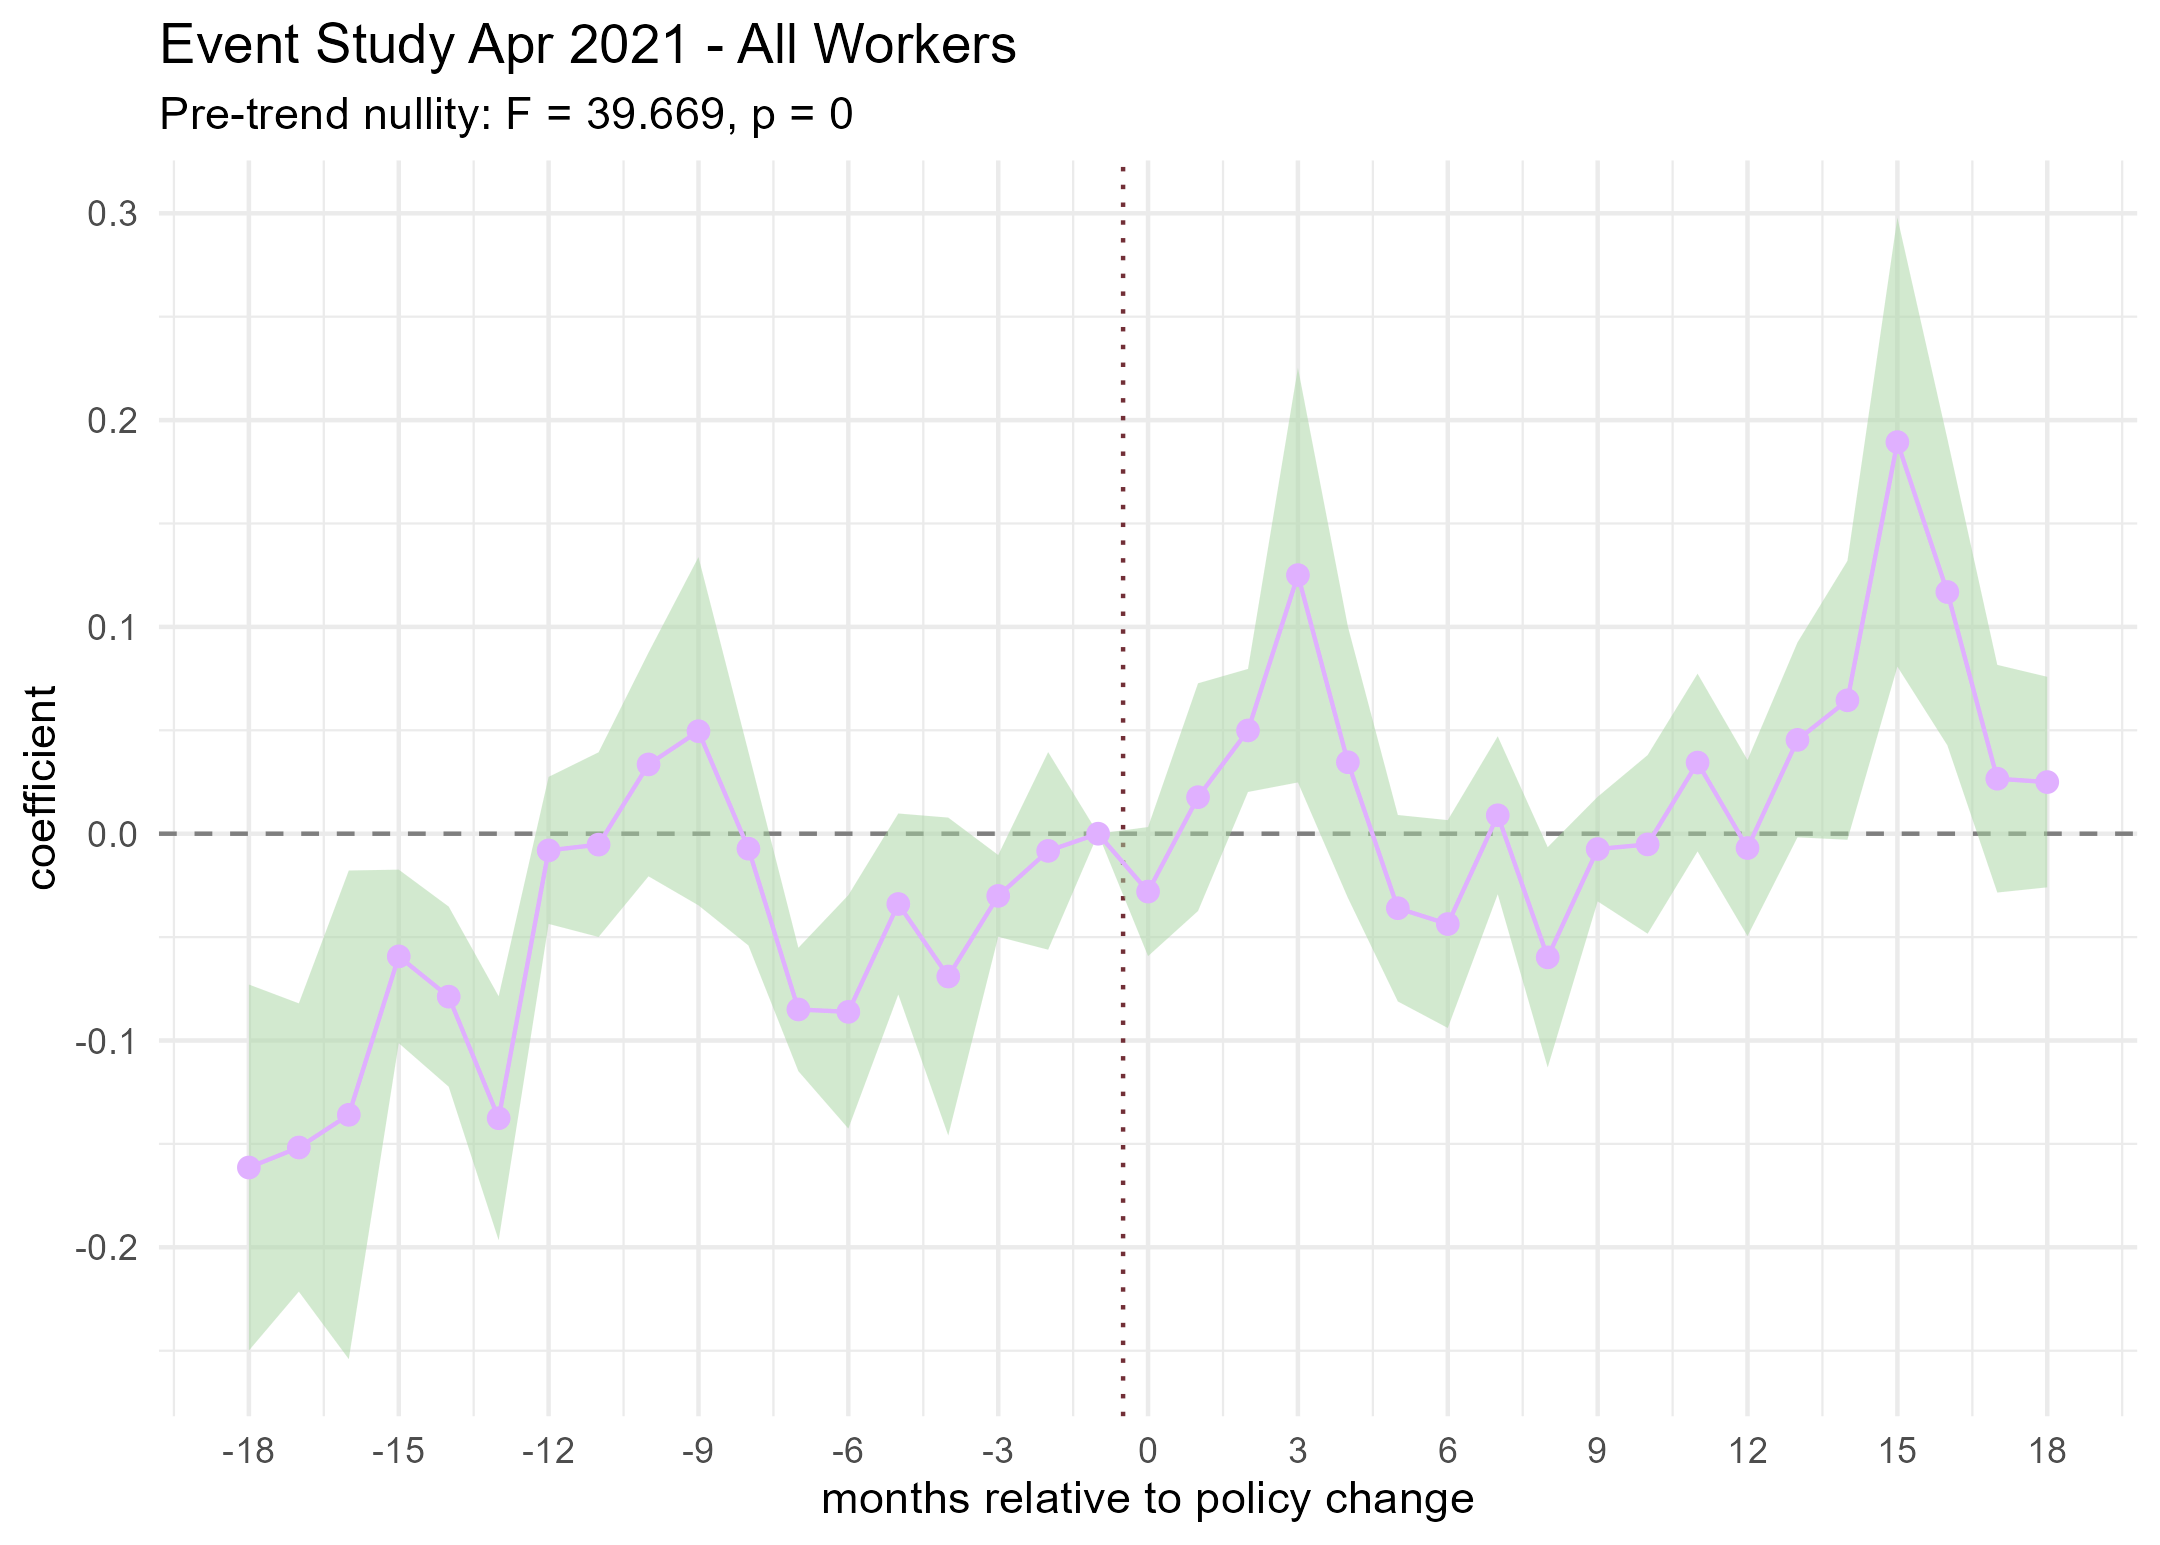
\includegraphics[width=\linewidth]{../../03 Output/DiD/event_study_2021.png}
\end{subfigure}\hfill
\begin{subfigure}{0.48\textwidth}
  \caption{French}
  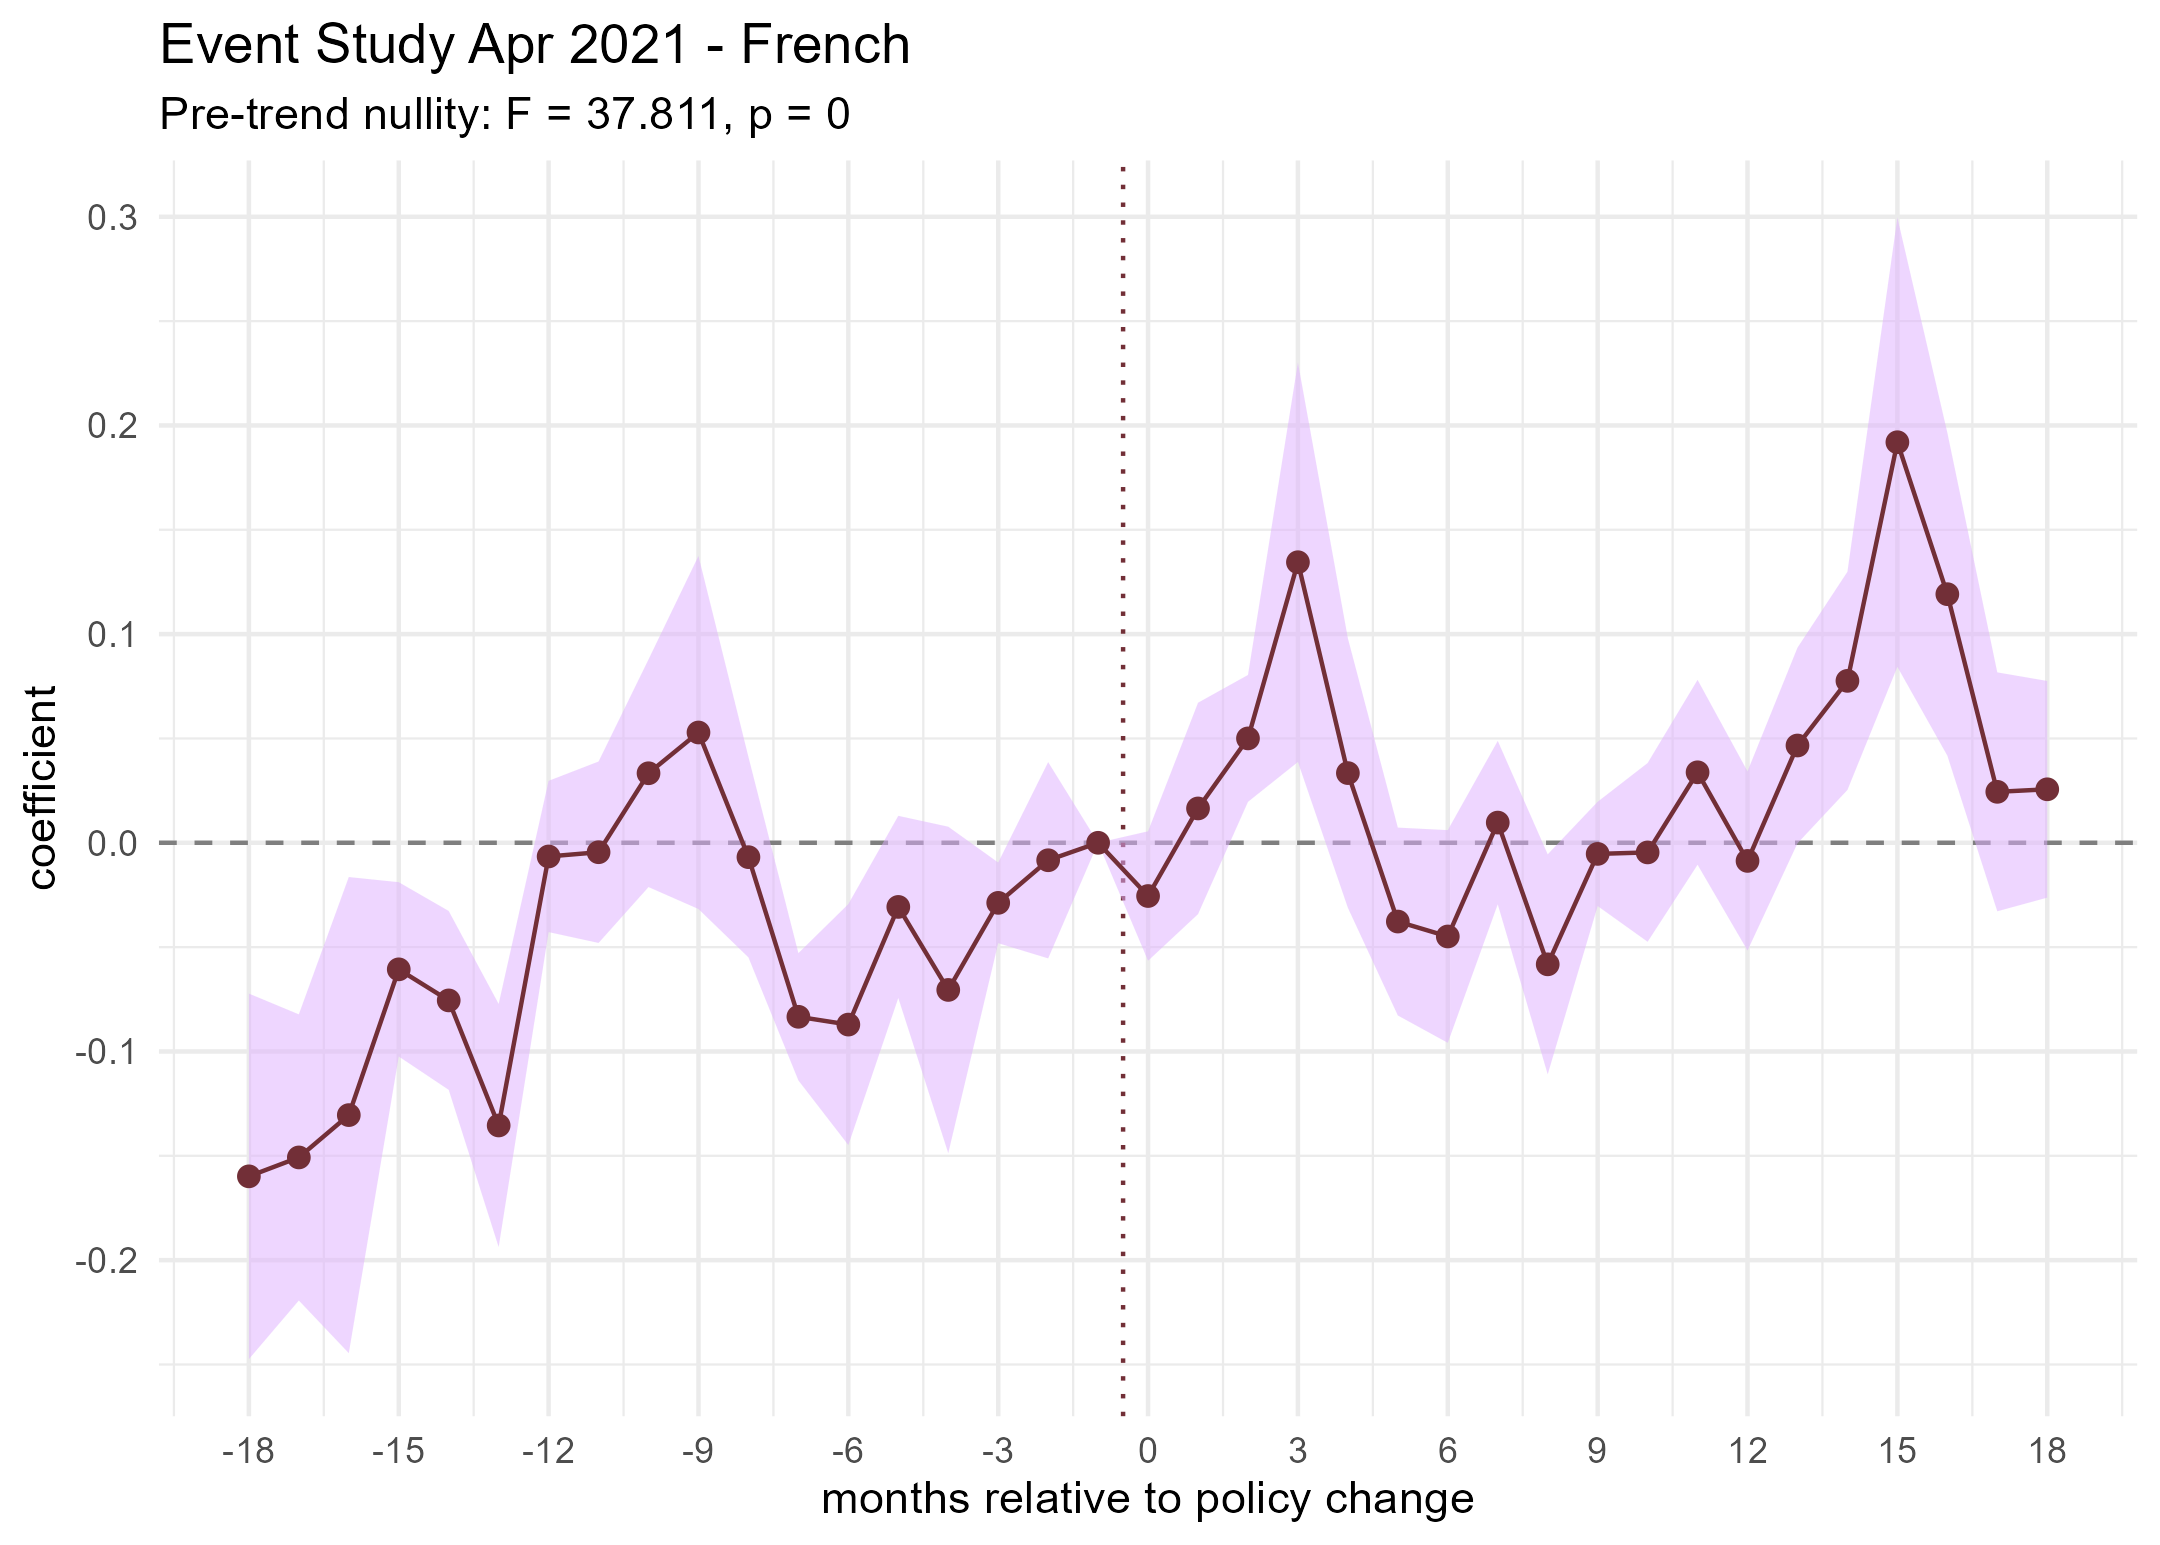
\includegraphics[width=\linewidth]{../../03 Output/DiD/event_study_french_2021.png}
\end{subfigure}
\par\medskip
\begin{subfigure}{0.48\textwidth}
  \caption{EEA}
  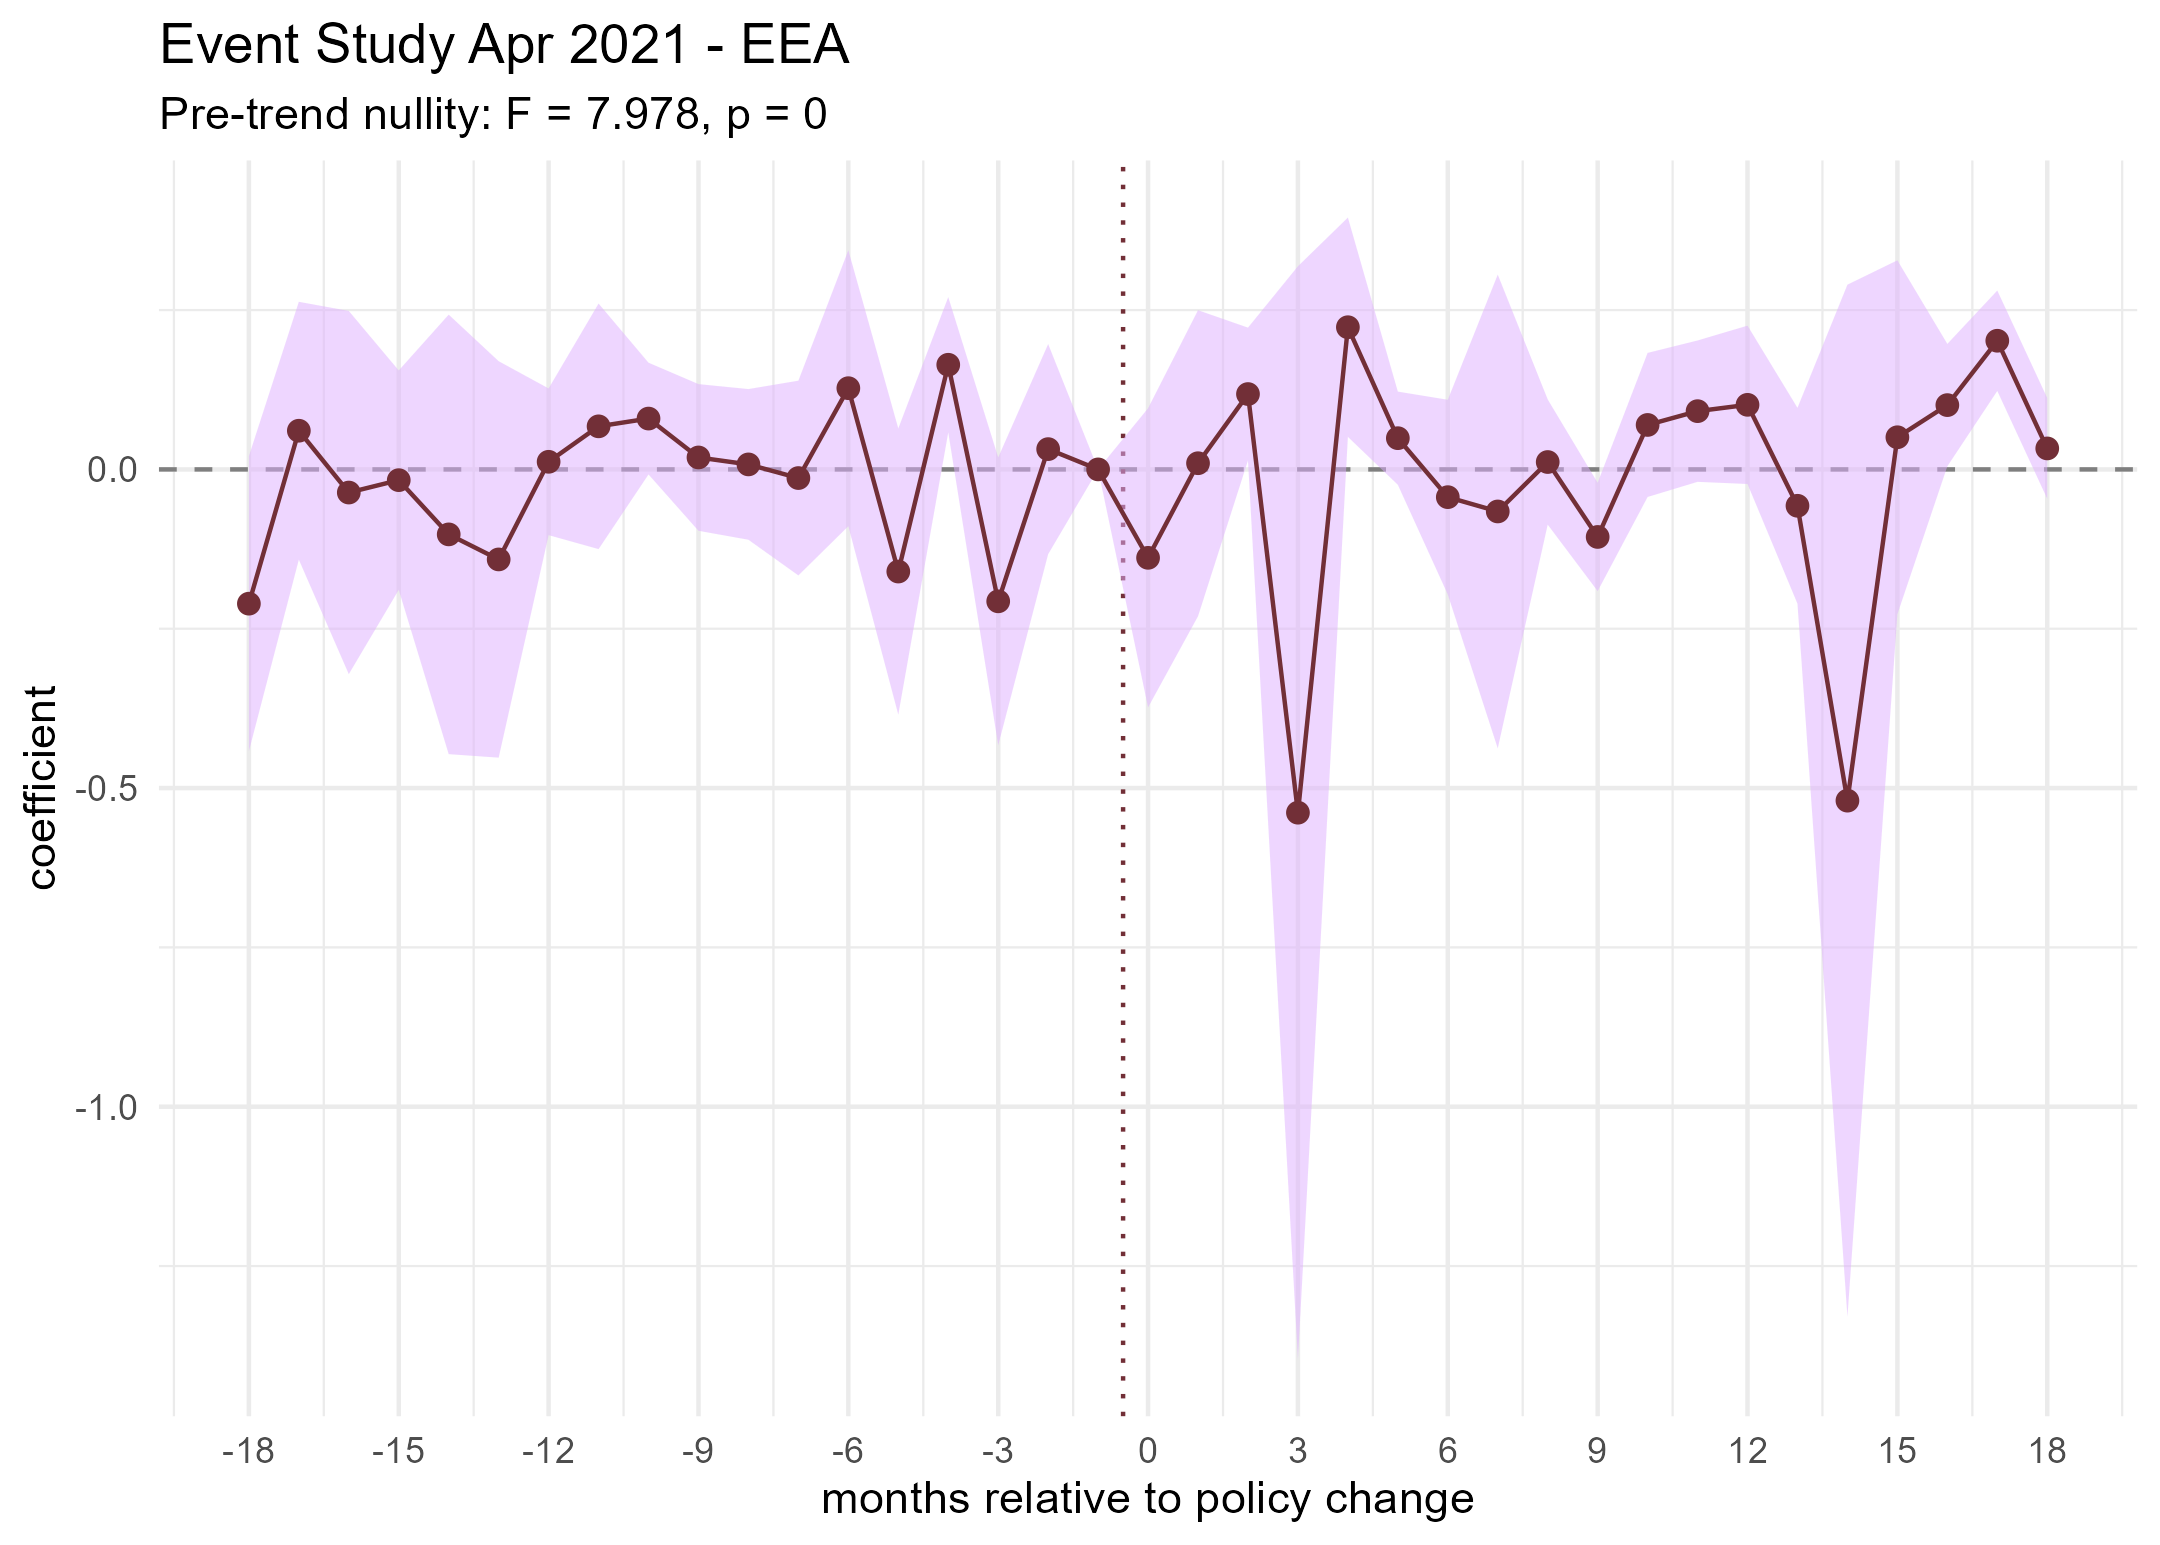
\includegraphics[width=\linewidth]{../../03 Output/DiD/event_study_eea_2021.png}
\end{subfigure}\hfill
\begin{subfigure}{0.48\textwidth}
  \caption{Non-EEA}
  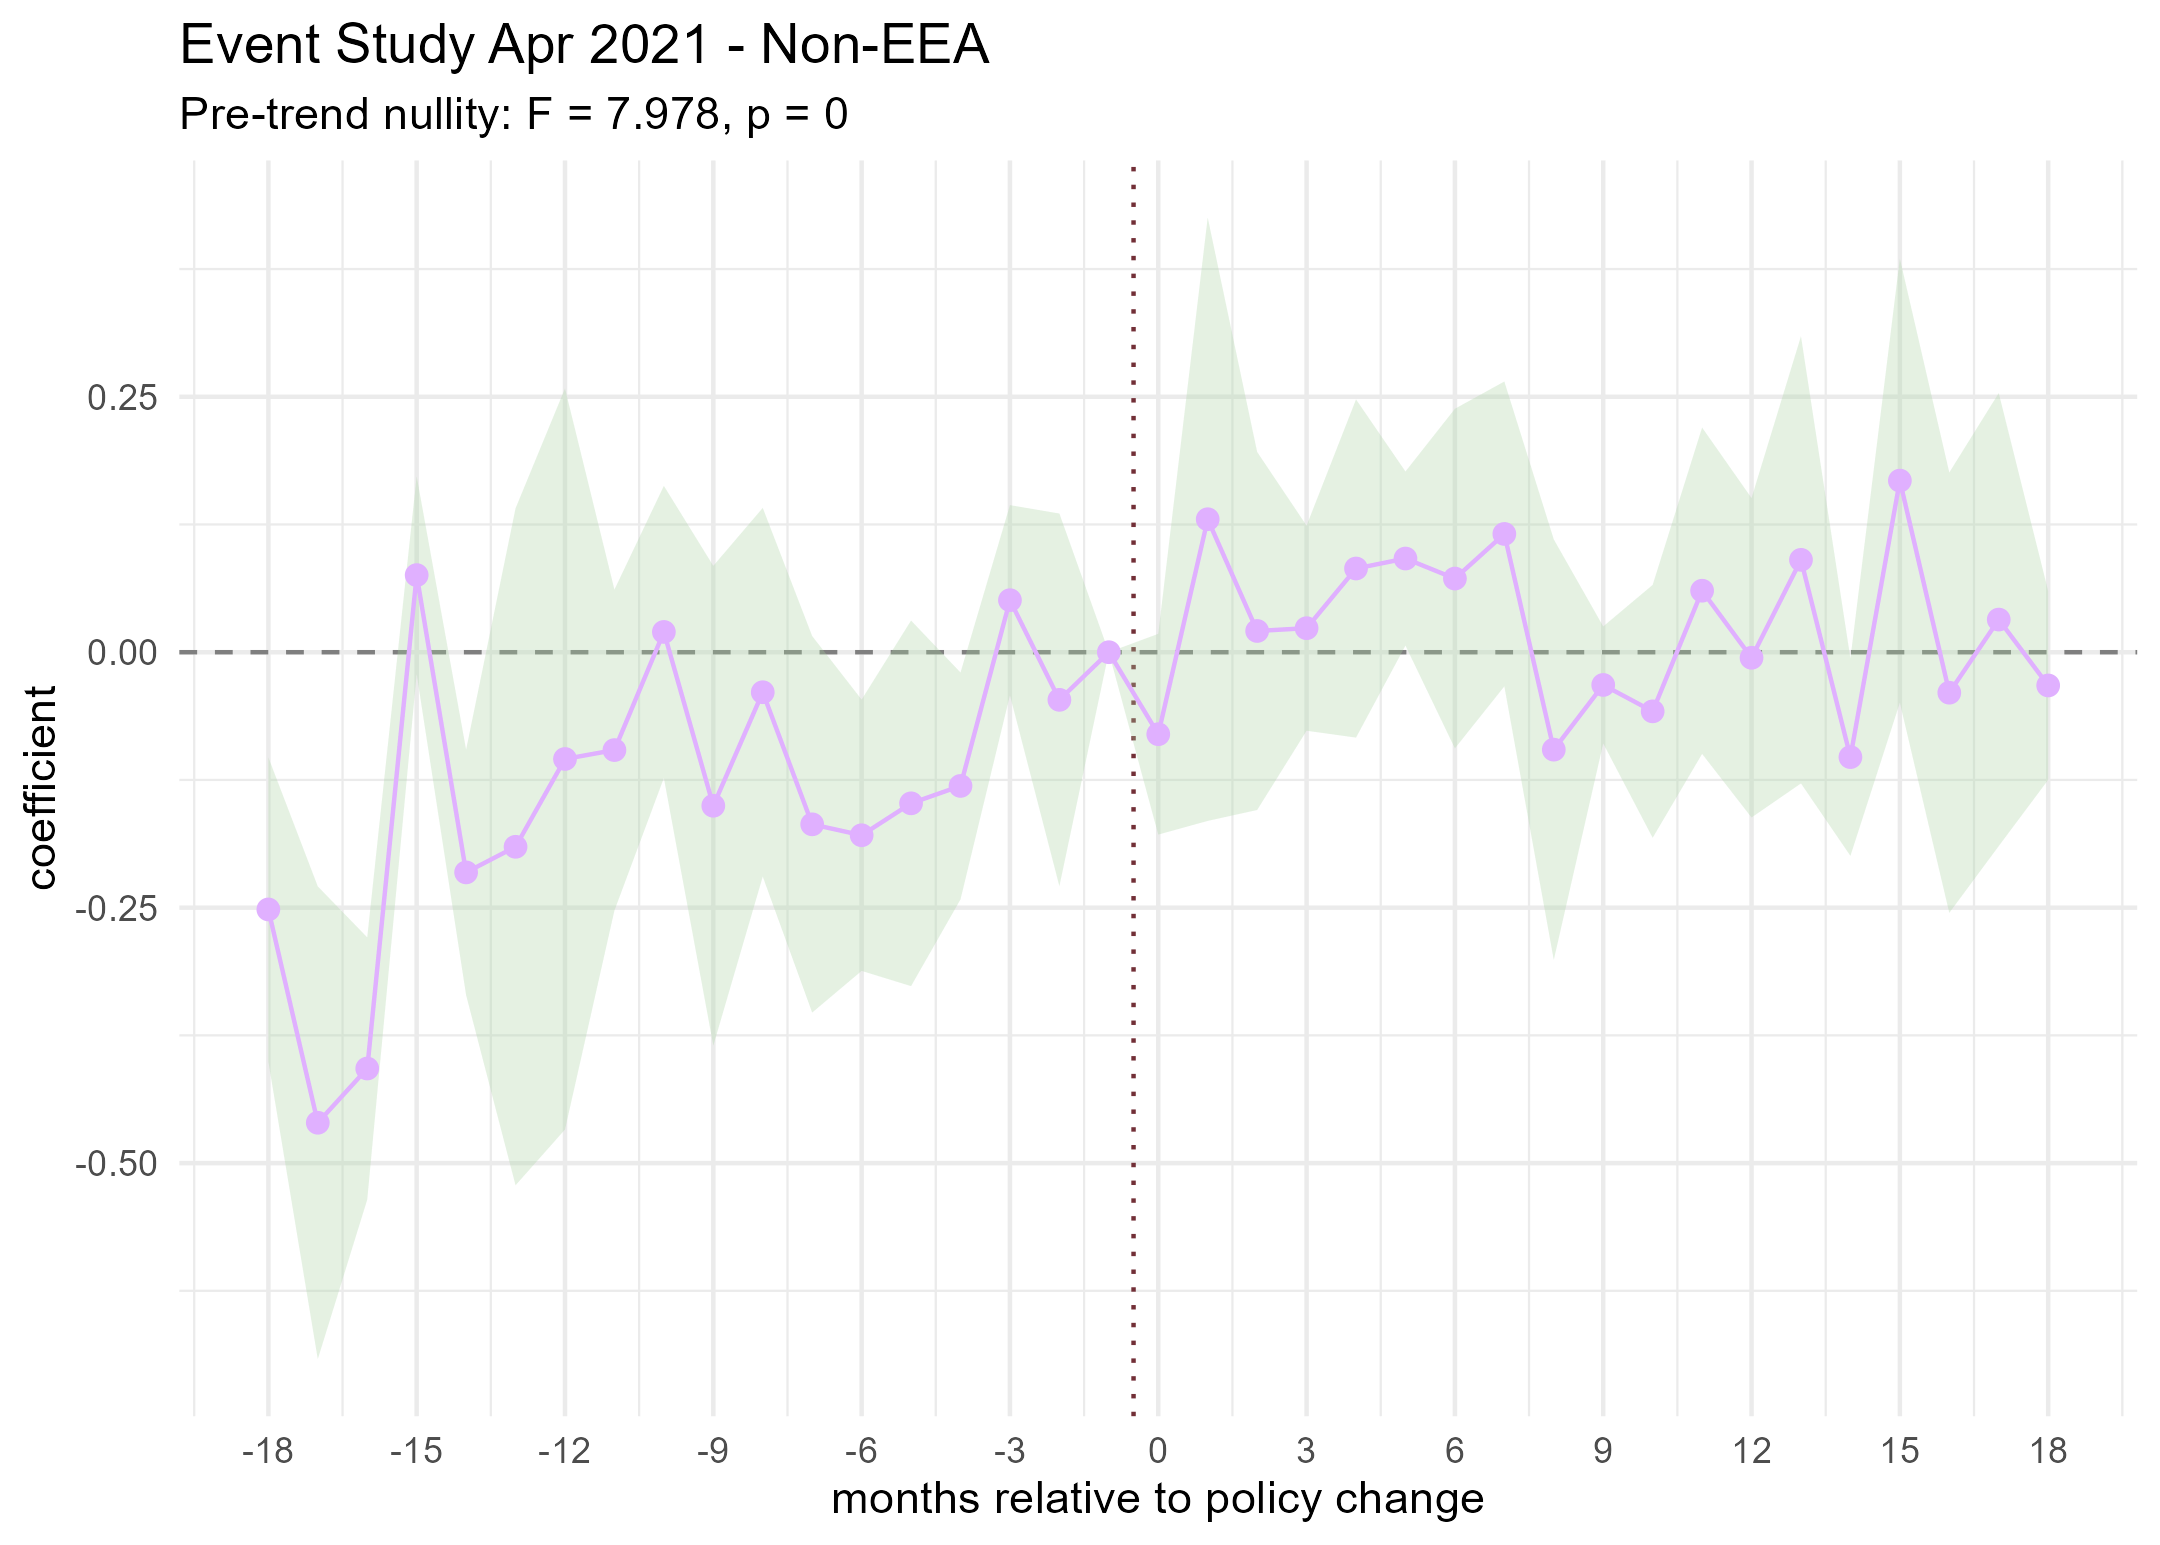
\includegraphics[width=\linewidth]{../../03 Output/DiD/event_study_non_eea_2021.png}
\end{subfigure}
\par\smallskip
{\footnotesize FE3 specification ($\mathtt{fap\_code \times year + region \times year}$), $\pm18$-month window. 95\% confidence intervals, SEs  clustered at FAP level.}
\end{figure}

\begin{table}[H]
\caption{2021 Reform (FE3)\label{tab:did2021_fe3}}
\centering
\setlength{\tabcolsep}{25pt}
\begin{tabular}{l|rrrr}
 & \textit{all} & \textit{french} & \textit{EEA} & \textit{non-EEA} \\
\midrule
\midrule
Treatment & $0.013$ & $0.013$ & $0.047$ & $-0.048^{*}$ \\
 & (0.014) & (0.014) & (0.044) & (0.028) \\[2pt]
Post & $0.019^{*}$ & $0.019^{*}$ & $0.035$ & $-0.004$ \\
 & (0.011) & (0.011) & (0.028) & (0.023) \\[2pt]
Treat$\,\times\,$Post & $-0.031$ & $-0.031$ & $-0.127$ & $0.051$ \\
 & (0.020) & (0.019) & (0.081) & (0.043) \\[2pt]
\midrule
Age & $0.002^{***}$ & $0.002^{***}$ & $-0.000$ & $-0.000$ \\
 & (0.000) & (0.000) & (0.001) & (0.001) \\[2pt]
Diploma & $0.025^{***}$ & $0.025^{***}$ & $0.028^{*}$ & $0.011$ \\
 & (0.003) & (0.003) & (0.015) & (0.013) \\[2pt]
Part-time & $-0.712^{***}$ & $-0.710^{***}$ & $-0.669^{***}$ & $-0.833^{***}$ \\
 & (0.024) & (0.024) & (0.040) & (0.052) \\[2pt]
Education & $-0.008^{**}$ & $-0.009^{**}$ & $-0.002$ & $0.003^{*}$ \\
 & (0.004) & (0.004) & (0.003) & (0.002) \\[2pt]
Male & $0.048^{**}$ & $0.048^{**}$ & $0.067^{***}$ & $0.085^{**}$ \\
 & (0.023) & (0.023) & (0.023) & (0.034) \\[2pt]
\midrule
Observations & 2{,}284{,}890 & 2{,}241{,}143 & 16{,}173 & 27{,}574 \\
\bottomrule
\multicolumn{5}{p{0.88\linewidth}}{\footnotesize Fixed effects: \texttt{fap\_code $\times$ year + region $\times$ year}. SEs clustered at FAP level. $^{***}p<0.01$, $^{**}p<0.05$, $^{*}p<0.10$.}\\
\end{tabular}
\end{table}
\clearpage

\begin{table}[h!]
\caption{2025 Reform (FE3)\label{tab:did2025_fe3}}
\centering
\setlength{\tabcolsep}{25pt}
\begin{tabular}{lrrrr}
 & \textit{all} & \textit{french} & \textit{EEA} & \textit{non-EEA} \\
\midrule
\midrule
Treatment & $0.002$ & $0.001$ & $-0.051$ & $0.028^{*}$ \\
 & (0.015) & (0.015) & (0.040) & (0.017) \\[2pt]
Post & $0.007$ & $0.007$ & $-0.014$ & $0.025$ \\
 & (0.011) & (0.010) & (0.020) & (0.021) \\[2pt]
Treat$\,\times\,$Post & $-0.007$ & $-0.008$ & $0.031$ & $0.012$ \\
 & (0.013) & (0.014) & (0.030) & (0.021) \\[2pt]
\midrule
Age & $-0.001$ & $-0.001$ & $-0.001$ & $-0.001^{*}$ \\
 & (0.000) & (0.000) & (0.001) & (0.001) \\[2pt]
Diploma & $0.004$ & $0.005$ & $-0.015$ & $0.011$ \\
 & (0.003) & (0.003) & (0.019) & (0.013) \\[2pt]
Part-time & $-0.802^{***}$ & $-0.802^{***}$ & $-0.699^{***}$ & $-0.911^{***}$ \\
 & (0.034) & (0.033) & (0.062) & (0.051) \\[2pt]
Education & $0.004$ & $0.005$ & $0.007$ & $0.004$ \\
 & (0.003) & (0.003) & (0.004) & (0.003) \\[2pt]
Male & $0.064^{**}$ & $0.065^{**}$ & $0.042$ & $0.091^{***}$ \\
 & (0.027) & (0.028) & (0.028) & (0.033) \\[2pt]
\midrule
Observations & 583{,}337 & 567{,}507 & 6{,}332 & 9{,}498 \\
\bottomrule
\multicolumn{5}{p{0.88\linewidth}}{\footnotesize Fixed effects: \texttt{fap\_code $\times$ year + region $\times$ year}. SEs clustered at FAP level. $^{***}p<0.01$, $^{**}p<0.05$, $^{*}p<0.10$.}\\
\end{tabular}
\end{table}

\begin{table}[h!]
\caption{Composition (FE1)\label{tab:selection}}
\centering
\setlength{\tabcolsep}{25pt}
\begin{tabular}{lrrr}
 & \textit{french} & \textit{EEA} & \textit{non-EEA} \\
\midrule
\multicolumn{4}{l}{\textit{Panel A: 2021 reform}} \\[3pt]
Treatment & $0.045^{**}$ & $0.167$ & $-0.241^{*}$ \\
 & (0.021) & (0.162) & (0.129) \\[2pt]
Post & $0.005$ & $-0.035$ & $0.090^{*}$ \\
 & (0.025) & (0.086) & (0.051) \\[2pt]
Treat$\,\times\,$Post & $-0.014$ & $-0.037$ & $0.117$ \\
 & (0.017) & (0.101) & (0.081) \\[2pt]
\midrule
Observations & 2{,}439{,}871 & 17{,}004 & 28{,}835 \\
\midrule
\multicolumn{4}{l}{\textit{Panel B: 2025 reform}} \\[3pt]
Treatment & $-0.024$ & $0.021$ & $0.069$ \\
 & (0.023) & (0.146) & (0.087) \\[2pt]
Post & $0.001$ & $-0.026$ & $0.098$ \\
 & (0.015) & (0.127) & (0.080) \\[2pt]
Treat$\,\times\,$Post & $0.044^{*}$ & $0.170$ & $-0.098$ \\
 & (0.026) & (0.182) & (0.144) \\[2pt]
\midrule
Observations & 590{,}448 & 6{,}492 & 9{,}692 \\
\bottomrule
\multicolumn{4}{p{0.60\linewidth}}{\footnotesize Fixed effects: \texttt{fap\_code + region + year}. SEs clustered at FAP level. $^{***}p<0.01$, $^{**}p<0.05$, $^{*}p<0.10$.}\\
\end{tabular}
\end{table}

\medskip




% \noindent\textbf{Composition check.} The selection table (Table~\ref{tab:selection}) reports DiD estimates with workers' education score as the outcome, testing whether listing shifts the composition of new hires rather than wages. For the 2021 reform, no significant effect is found for any group, suggesting composition bias is unlikely to explain the wage estimates. For the 2025 reform, the French Treat$\,\times\,$Post coefficient is positive and marginally significant ($+0.044^{*}$), indicating a slight upward shift in the educational profile of French workers newly hired in listed occupations. No analogous pattern is detected for non-EEA or EEA workers, and the effect is too small to substantially distort the wage estimates.


\clearpage

\section{Conclusions}

\noindent \textit{Limitations} 
% - kimited time controls and FAP
% - not excluded those that had been treated
% - occupations listed since 2008 are excluded from both 
% treated and control groups to avoid contamination from long-standing listing effects. 
% - epople we work with do nto face much discrimination



\clearpage
\bibliography{biblio.bib}
\bibliographystyle{apalike}

\appendix
\clearpage
\section*{Appendix A - Descriptives}

\begin{table}[h]
\caption{Balance characteritics, by nationality group}
\vspace{0.2cm}
\label{tab:balance_status}
\centering
\small
\begin{tabular}{lrrr}
 & \textit{French} & \textit{EEA} & \textit{Non-EEA} \\
\midrule
\midrule
Individuals & 5{,}019{,}263 & 34{,}541 & 59{,}388 \\
Contracts   & 19{,}796{,}088 & 144{,}810 & 232{,}038 \\
\midrule
Monthly wage & 1{,}429 & 1{,}464$^{***}$ & 1{,}390$^{***}$ \\
Age                 & 32.0 & 35.2$^{***}$ & 37.4$^{***}$ \\
Male                & 0.499 & 0.502        & 0.555$^{***}$ \\
Part-time           & 0.223 & 0.234$^{***}$ & 0.294$^{***}$ \\
Experience (months) & 48    & 44$^{***}$   & 56$^{***}$ \\
Diploma         & 0.649 & 0.405$^{***}$ & 0.395$^{***}$ \\
Education (NIVFOR)  & 6.10  & 4.36$^{***}$ & 4.41$^{***}$ \\
\bottomrule
\end{tabular}
\par\vspace{2pt}
{\footnotesize Stars relate to $\neq$ from French ($^{***}p<0.01$, $^{**}p<0.05$, $^{*}p<0.10$).\\All EEA vs. non-EEA differences are significant at $p<0.05$.}
\end{table}

\begin{table}[h]
\caption{Balance characteristics - 2025 cohort}
\vspace{0.3cm}
\label{tab:balance_2025}
\centering
\setlength{\tabcolsep}{11pt}
\begin{tabular}{lrrrrrr}
 & \multicolumn{2}{c}{\textit{French}} & \multicolumn{2}{c}{\textit{EEA}} & \multicolumn{2}{c}{\textit{Non-EEA}} \\
\cmidrule(lr){2-3}\cmidrule(lr){4-5}\cmidrule(lr){6-7}
 & Unlisted & Listed & Unlisted & Listed & Unlisted & Listed \\
\midrule
\midrule
Individuals & 4{,}409{,}213 & 610{,}050 & 29{,}033 & 5{,}508 & 44{,}706 & 14{,}682 \\
Contracts   & 17{,}071{,}372 & 2{,}724{,}716 & 118{,}605 & 26{,}205 & 167{,}625 & 64{,}413 \\
\midrule
Monthly wage & 1{,}423 & 1{,}457$^{***}$ & 1{,}435 & 1{,}572$^{***}$ & 1{,}326 & 1{,}537$^{***}$ \\
Age  & 32.0 & 32.4$^{***}$ & 35.0 & 36.0$^{***}$ & 37.1 & 38.3$^{***}$ \\
Male & 0.493 & 0.540$^{***}$ & 0.497 & 0.529$^{***}$ & 0.534 & 0.618$^{***}$ \\
Part-time           & 0.215 & 0.280$^{***}$ & 0.220 & 0.304$^{***}$ & 0.285 & 0.307$^{***}$ \\
Experience (months) & 48    & 46$^{***}$    & 44    & 45            & 55    & 61$^{***}$ \\
Diploma         & 0.656 & 0.599$^{***}$ & 0.412 & 0.367$^{***}$ & 0.416 & 0.330$^{***}$ \\
Education (NIVFOR)  & 6.20  & 5.33$^{***}$  & 4.44  & 3.96$^{***}$  & 4.62  & 3.77$^{***}$ \\
\bottomrule
\multicolumn{7}{p{0.95\linewidth}}{\footnotesize Stars relate to $\neq$ between
listed and unlisted cells within each nationality group ($^{***}p<0.01$, $^{**}p<0.05$, $^{*}p<0.10$).}\\
\end{tabular}
\end{table}

\begin{figure}[h!]
\caption{Wage distribution, by nationality group}
\label{wage}
\vspace{0.2cm}
\centering
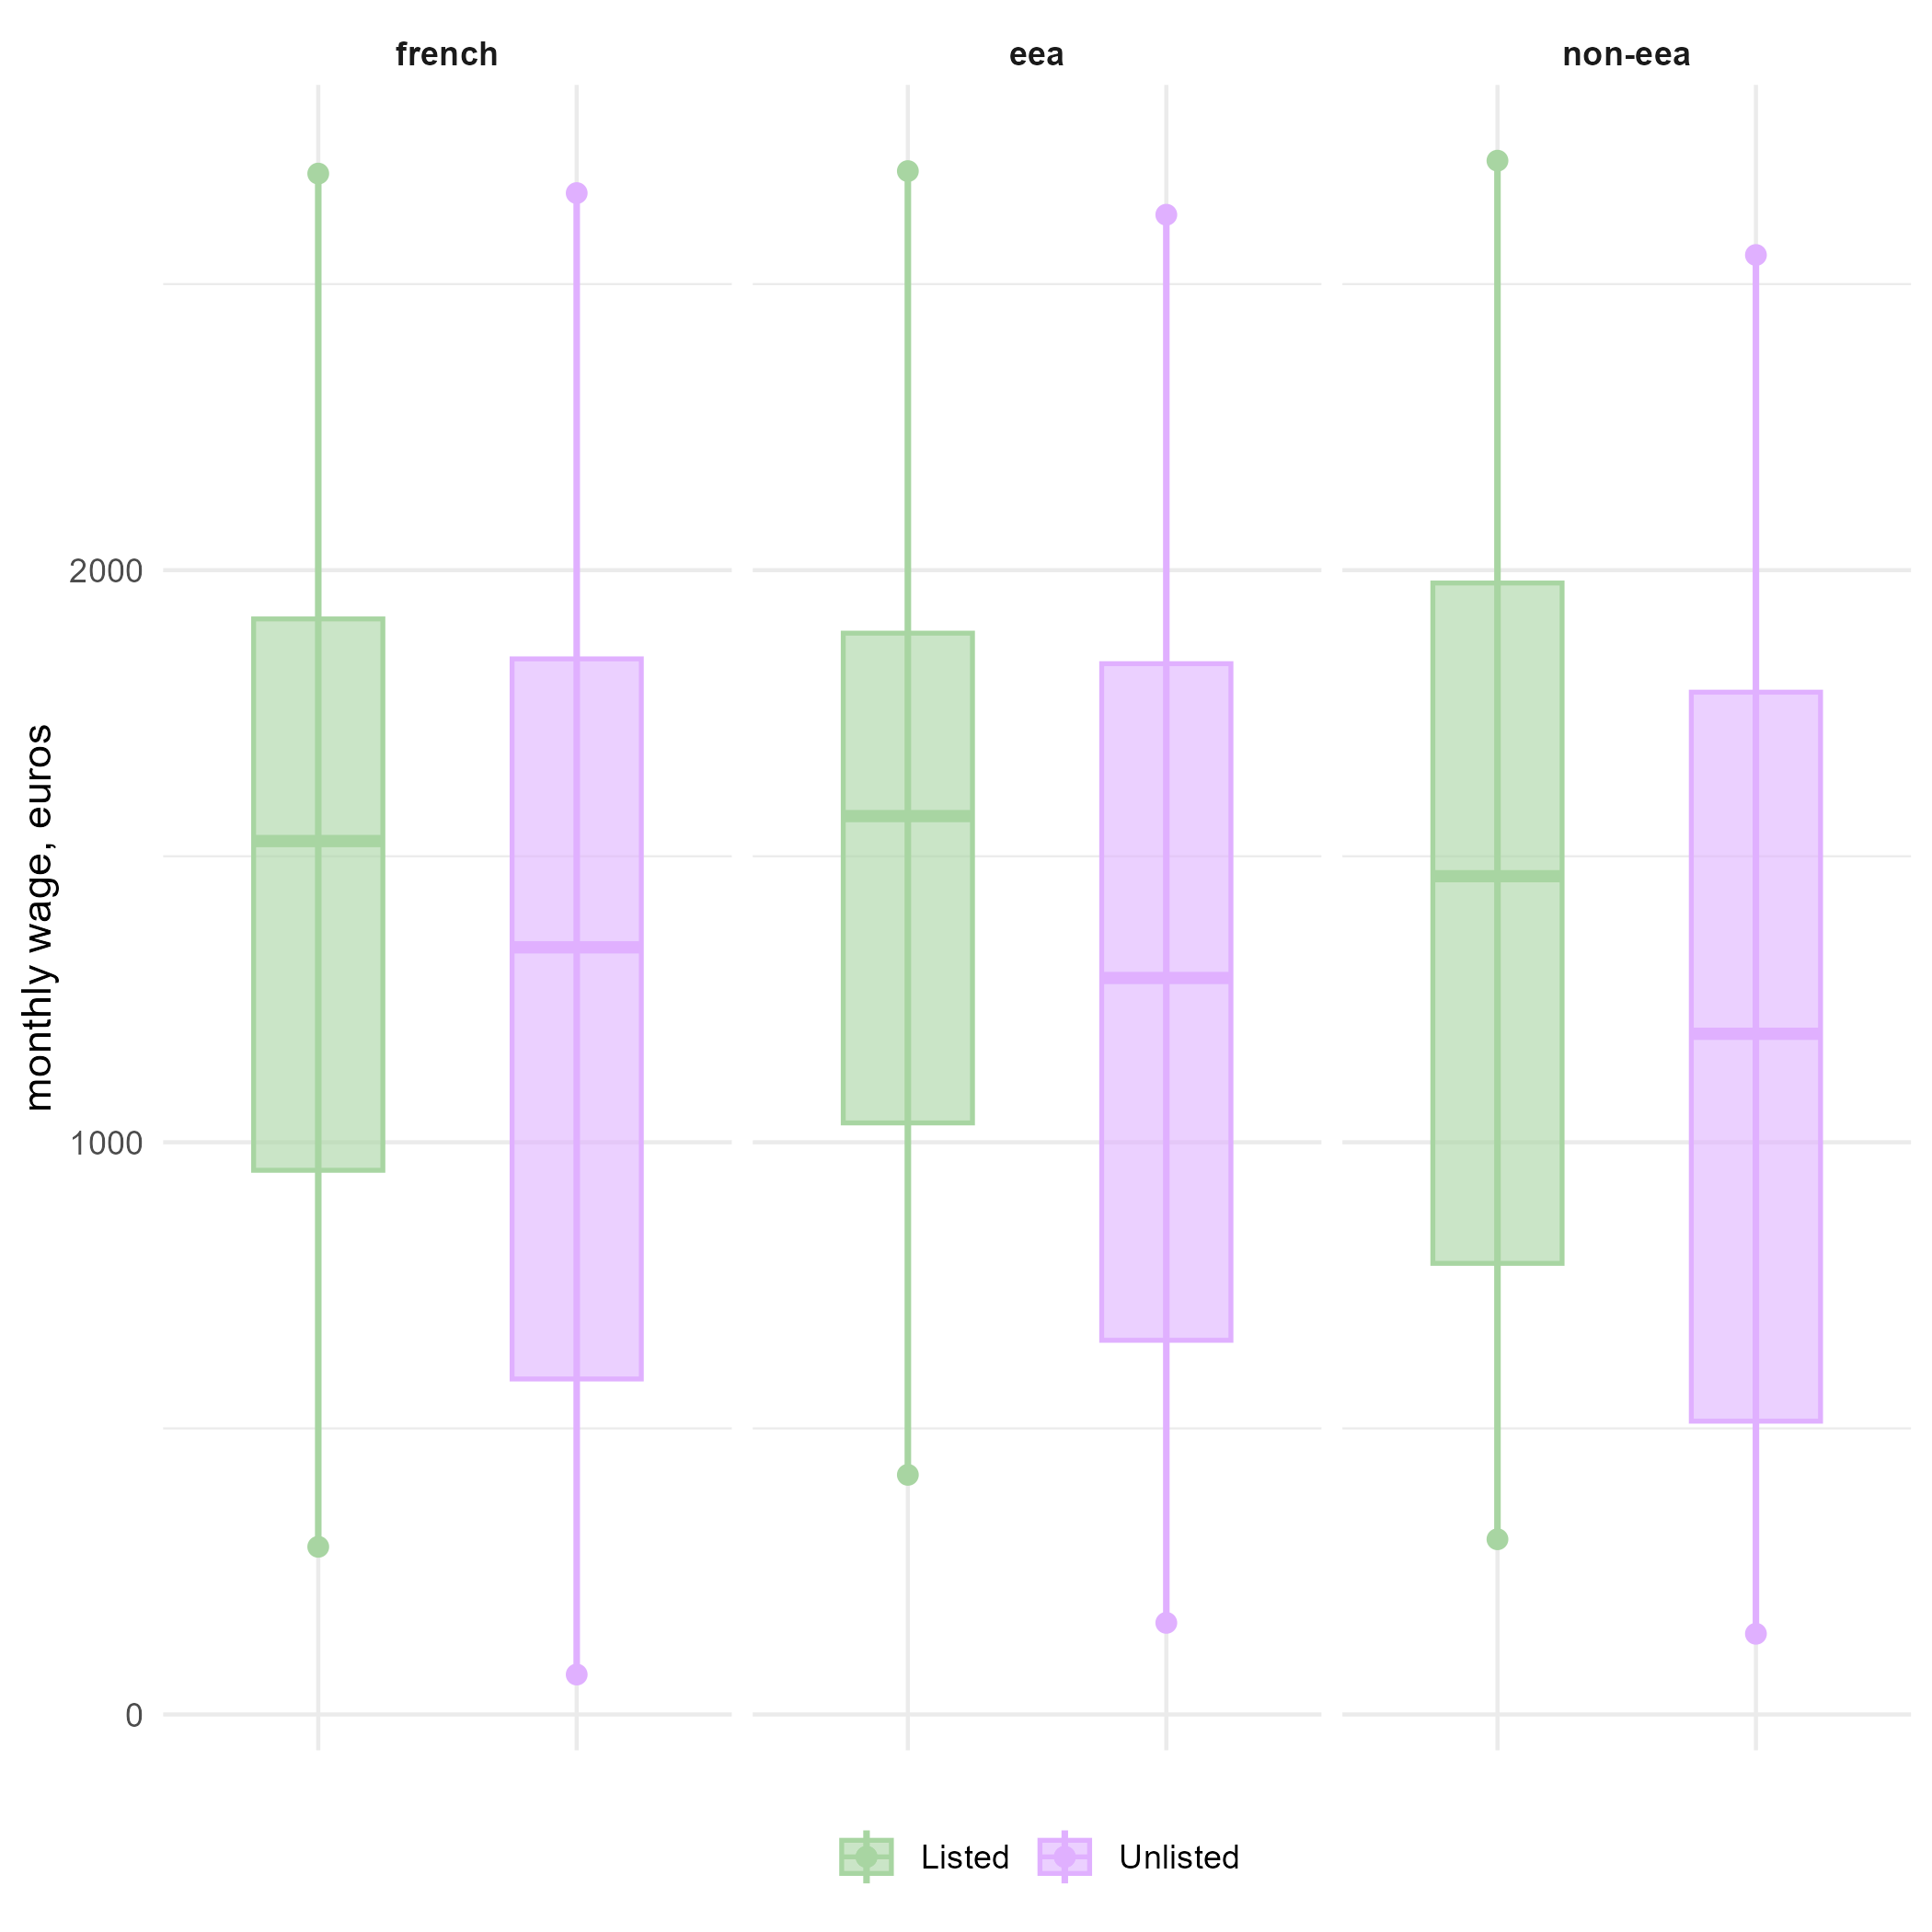
\includegraphics[width=0.5\textwidth]{../../03 Output/Descriptives/boxplot_fullsample.png}
\end{figure}

\begin{figure}[h!]
    \label{share}
\caption{Share of contracts, by nationality group}
\vspace{0.2cm}
\centering
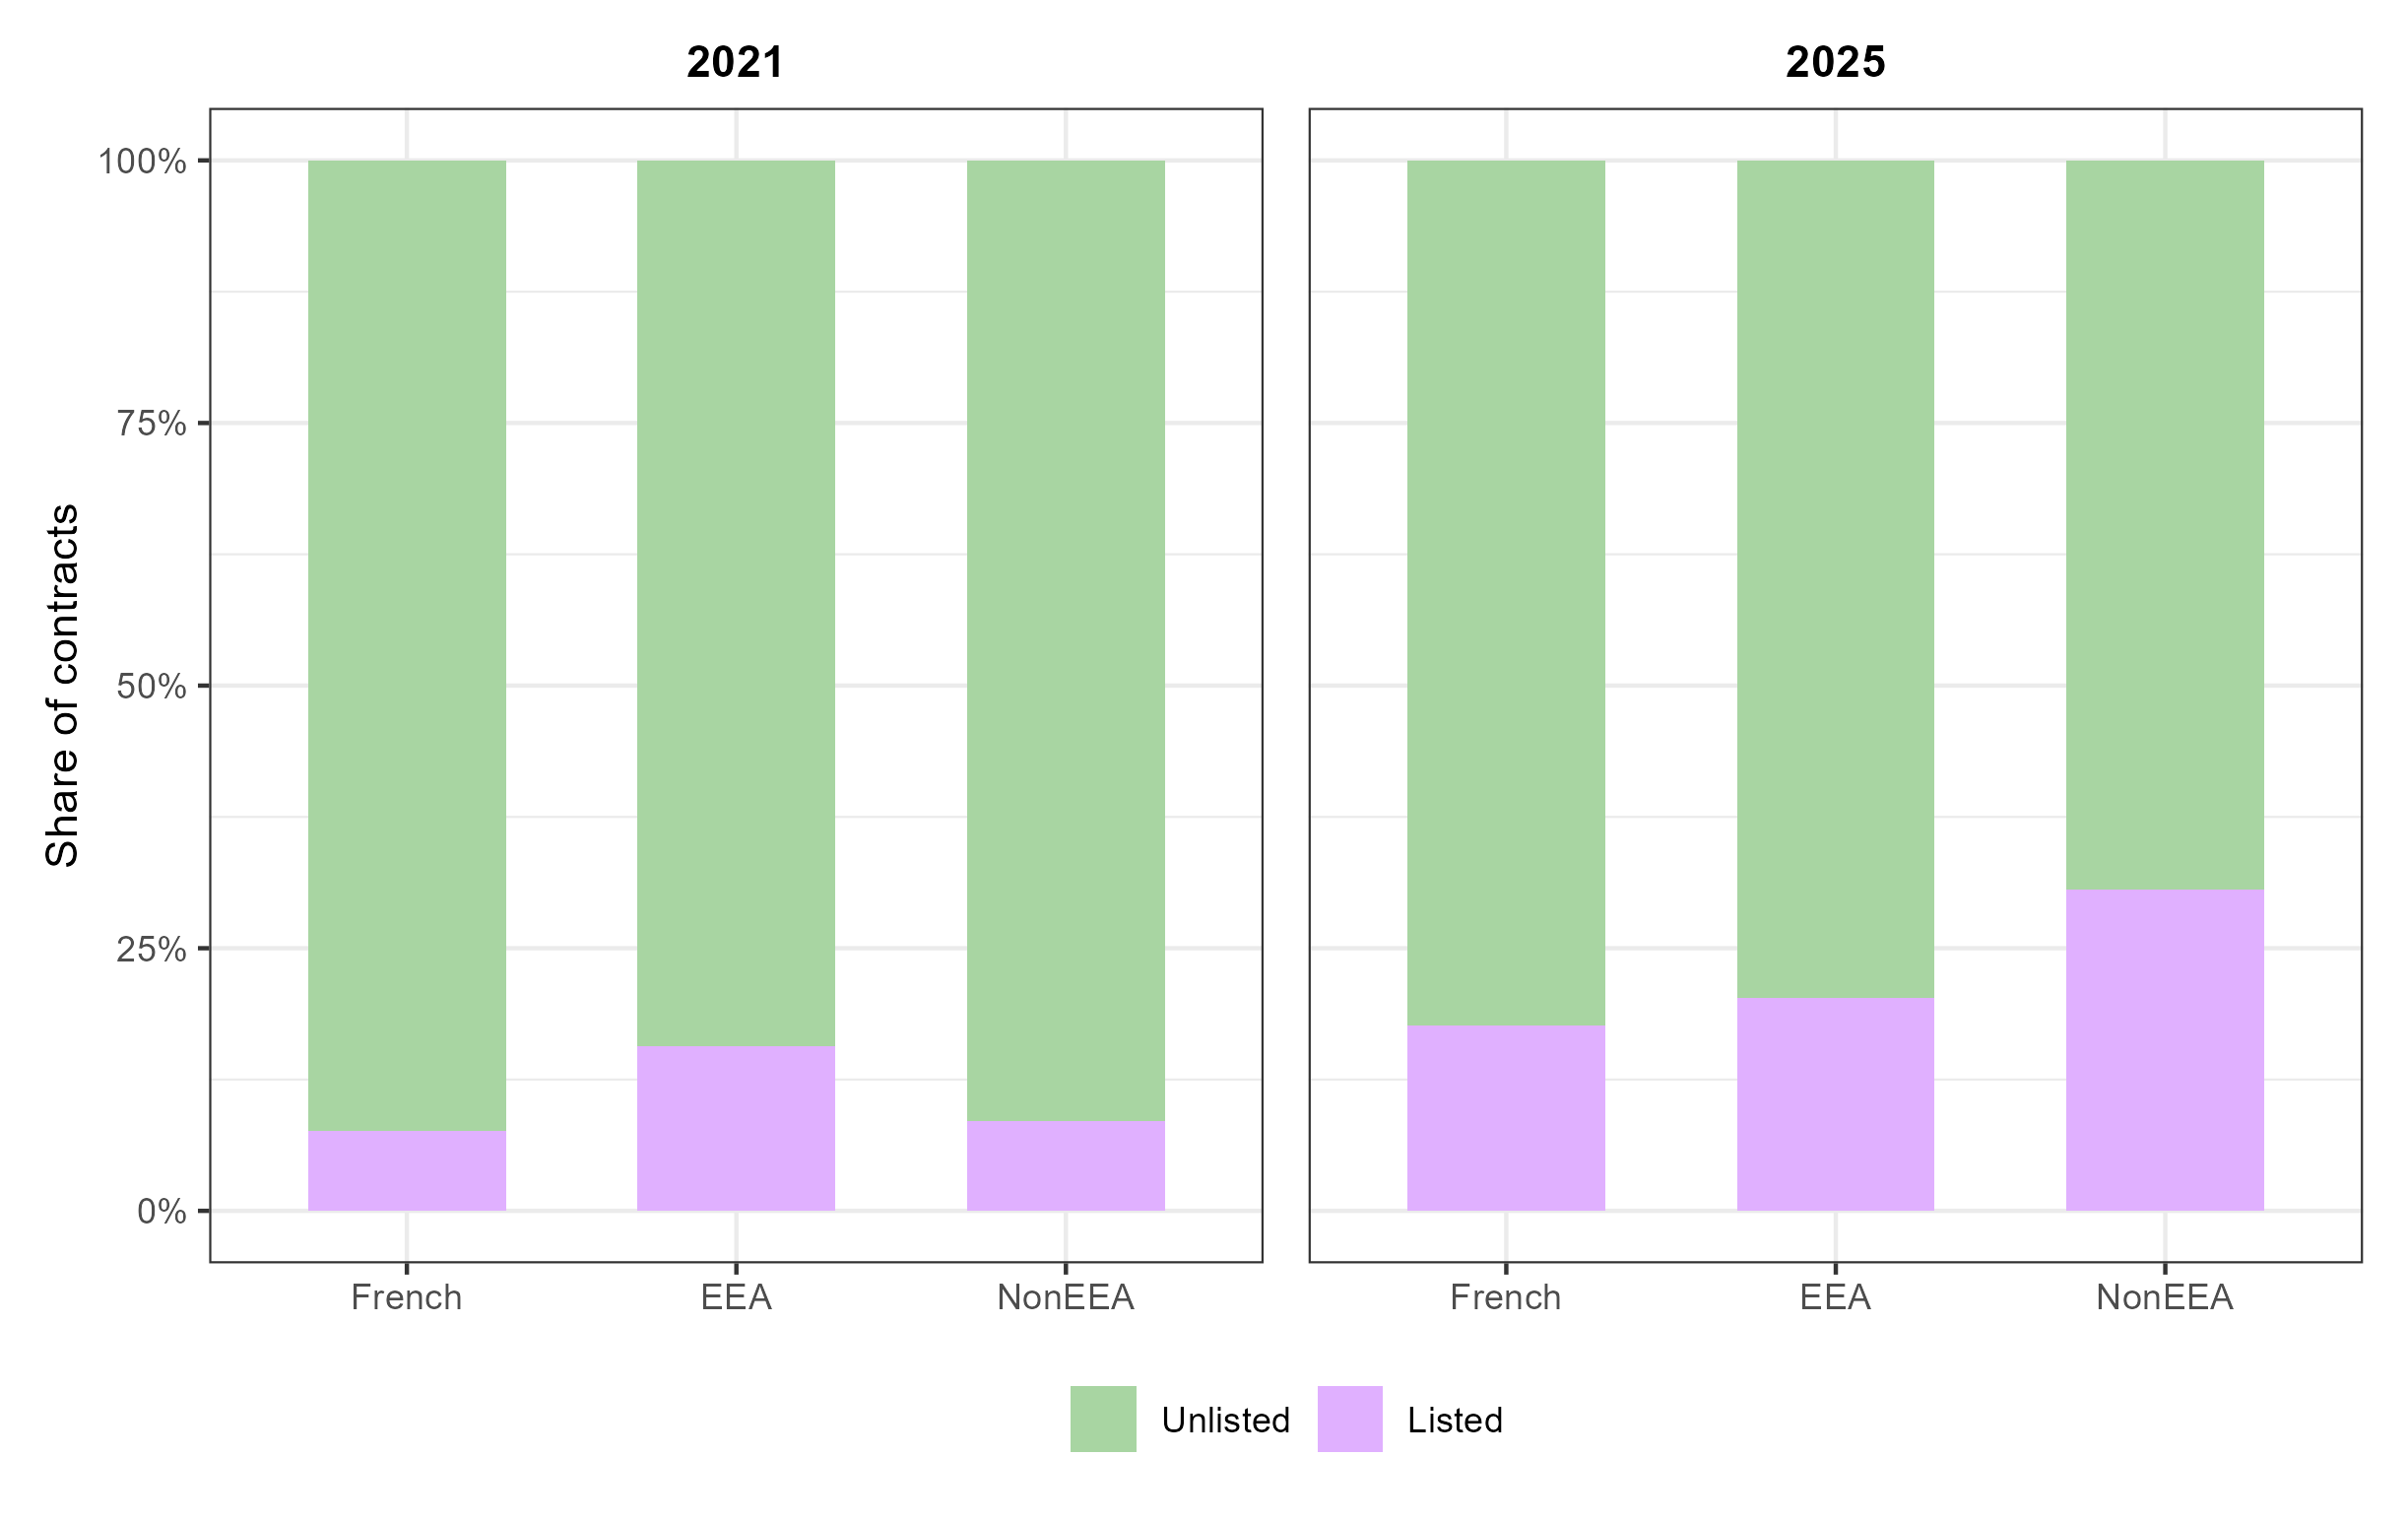
\includegraphics[width=0.7\textwidth]{../../03 Output/Descriptives/sharecontracts.png}
\end{figure}

\FloatBarrier
\section*{Appendix B - Shortage List}

\begin{table}[h!]
\caption{Listed FAP, by region and listing year}
\footnotesize
\label{listing}
\vspace{0.3cm}
\centering
\begin{tabular}{l|rrr|r}
\textit{region} & \textit{2021} & \textit{2024} & \textit{2025} & \textit{total} \\
  \midrule
Auvergne-Rhône-Alpes &  21 &   2 &  31 &  74 \\ 
  Nouvelle-Aquitaine &  24 &   2 &  28 &  74 \\ 
  Provence-Alpes-Côte d'Azur &  18 &   4 &  30 &  71 \\ 
  Bourgogne-Franche-Comté &  24 &   4 &  22 &  70 \\ 
  Centre-Val de Loire &  26 &   3 &  21 &  70 \\ 
  Grand Est &  16 &   4 &  25 &  69 \\ 
  Occitanie &  26 &   2 &  23 &  69 \\ 
  Pays de la Loire &  26 &   4 &  18 &  69 \\ 
  Hauts-de-France &  24 &   2 &  21 &  65 \\ 
  Normandie &  23 &   4 &  15 &  64 \\ 
  Île-de-France &  20 &   4 &  17 &  63 \\ 
  Bretagne &  27 &   3 &  14 &  57 \\ 
  Corse &  13 &   4 &  20 &  47 \\ 
   \bottomrule
\end{tabular}
\end{table}

\begin{figure}[H]
\caption{Heatmap of listed occupations}
\centering
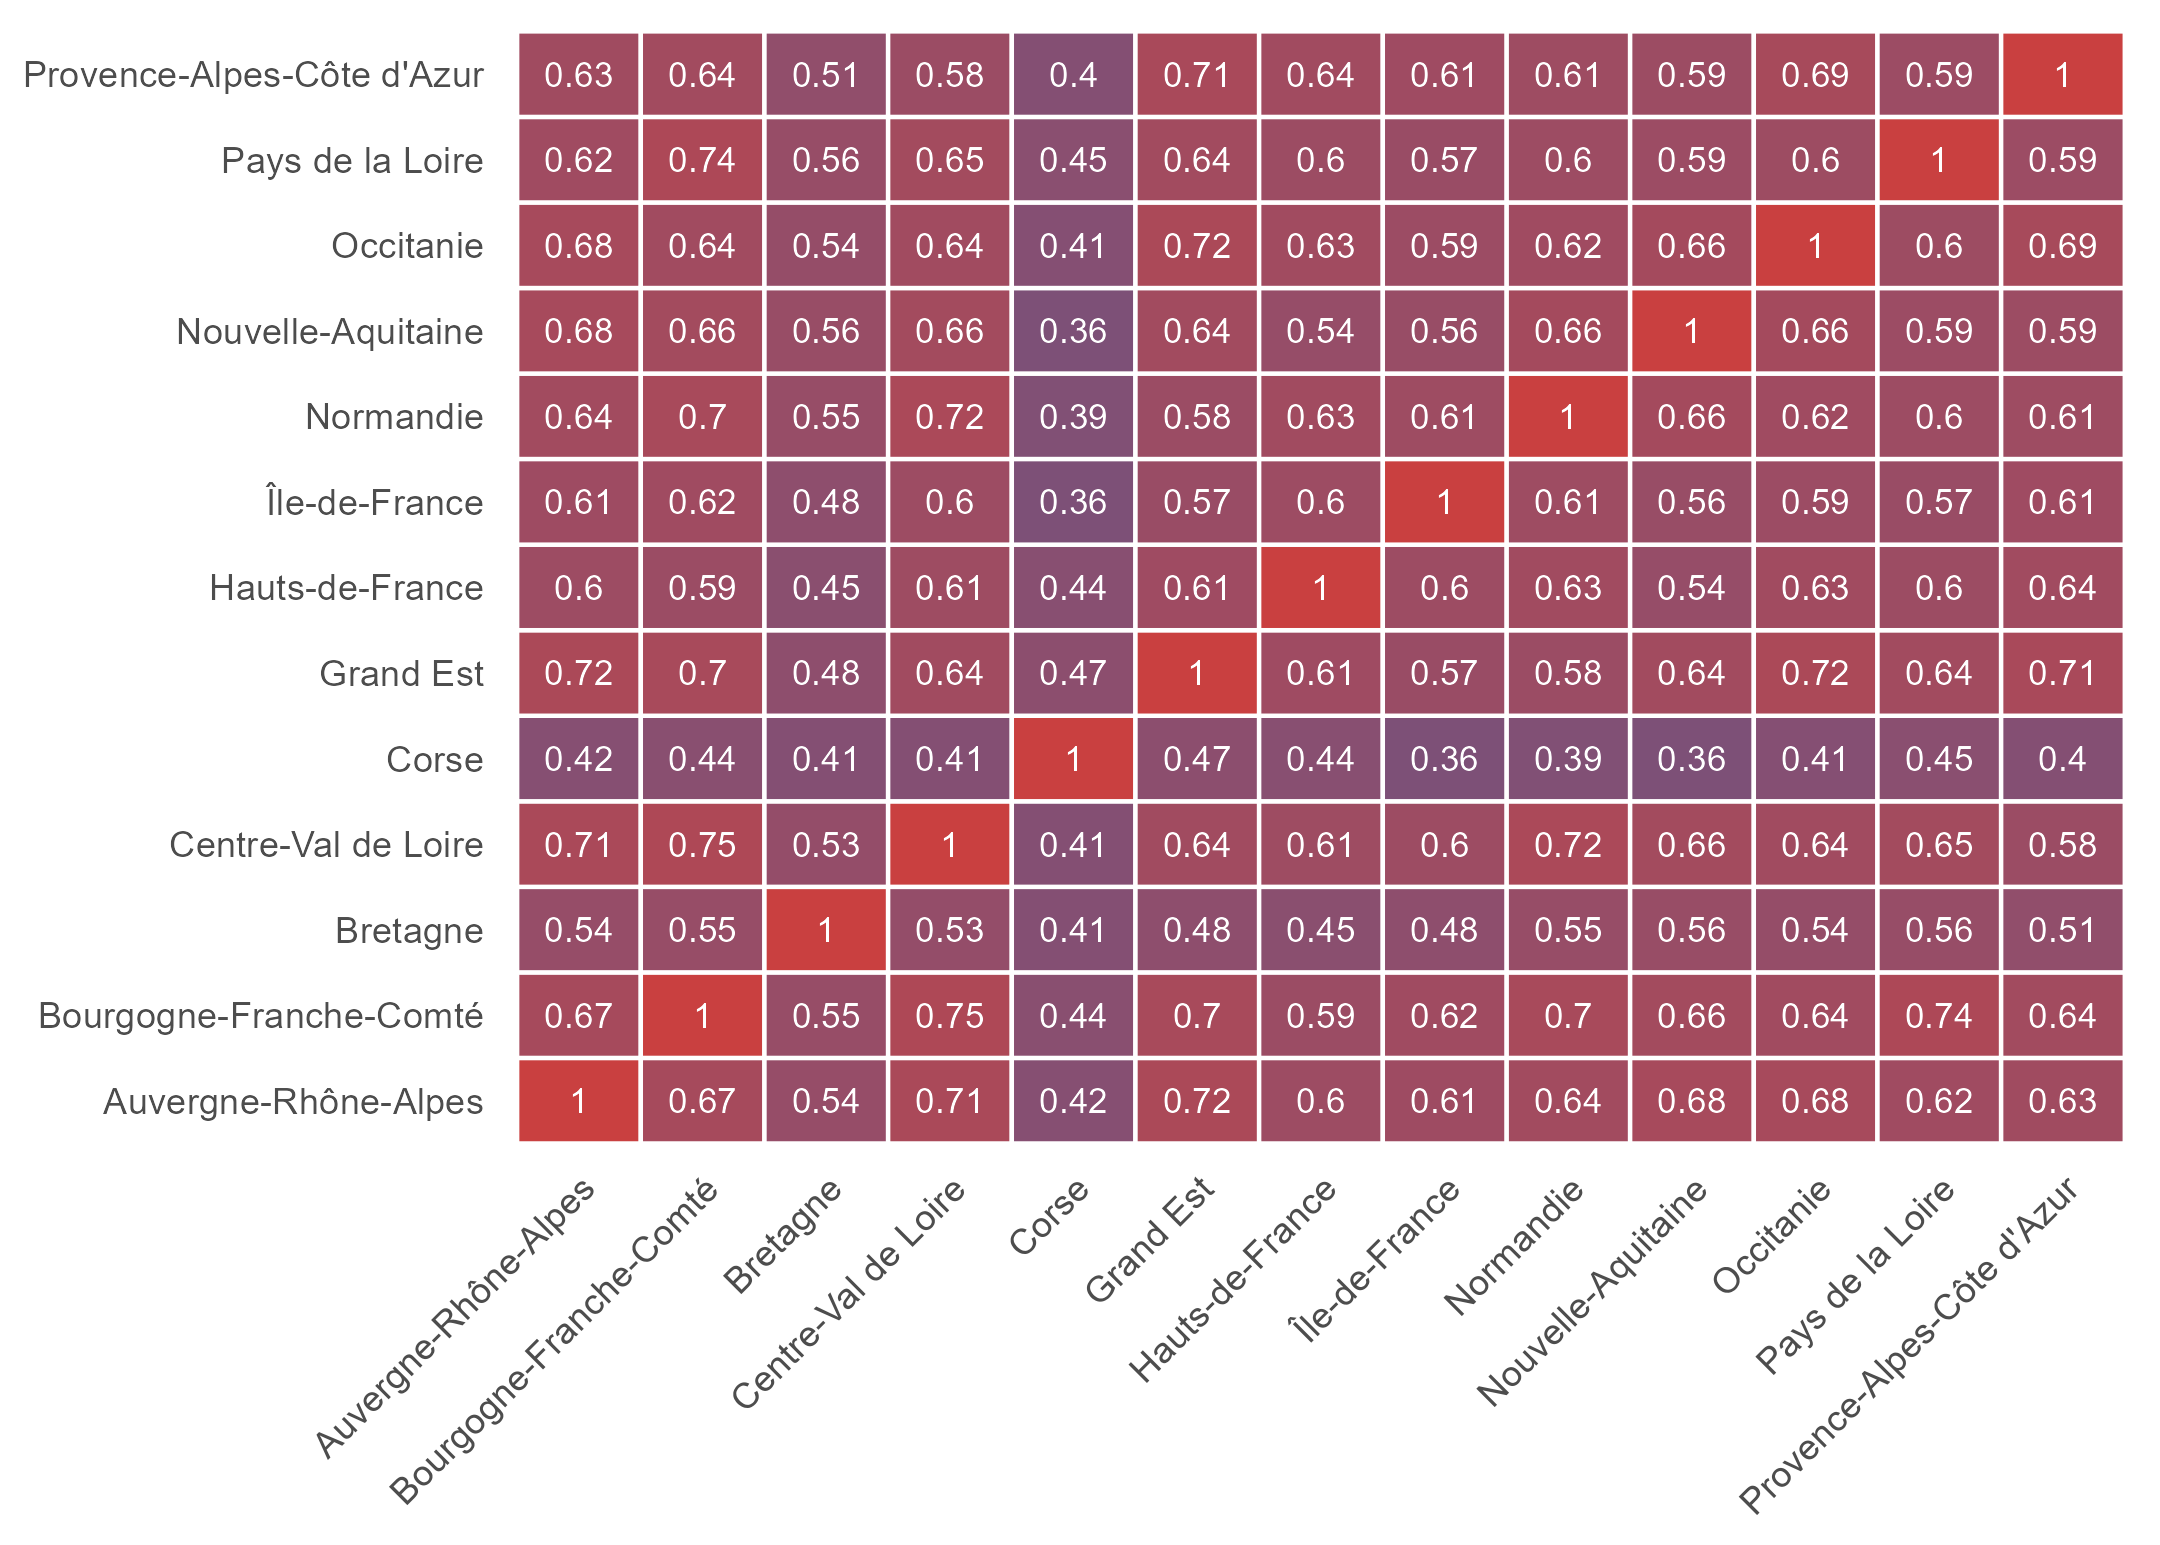
\includegraphics[width=0.6\textwidth]{../../03 Output/Descriptives/heatmap.png}
\end{figure}

\clearpage
\section*{Appendix C - Additional Results}

\begin{table}[h!]
\caption{2021 Reform (FE1)\label{tab:did2021_fe1}}
\centering
\setlength{\tabcolsep}{25pt}
\begin{tabular}{lrrrr}
 & \textit{all} & \textit{french} & \textit{EEA} & \textit{non-EEA} \\
\midrule
\midrule
Treatment & $0.006$ & $0.006$ & $0.028$ & $-0.047^{*}$ \\
 & (0.013) & (0.013) & (0.033) & (0.026) \\[2pt]
Post & $0.019$ & $0.019$ & $0.016$ & $-0.005$ \\
 & (0.012) & (0.012) & (0.027) & (0.024) \\[2pt]
Treat$\,\times\,$Post & $-0.018^{*}$ & $-0.018^{*}$ & $-0.088$ & $0.040$ \\
 & (0.010) & (0.009) & (0.072) & (0.032) \\[2pt]
\midrule
Age & $0.002^{***}$ & $0.003^{***}$ & $-0.000$ & $-0.000$ \\
 & (0.000) & (0.000) & (0.001) & (0.001) \\[2pt]
Diploma & $0.026^{***}$ & $0.026^{***}$ & $0.031^{**}$ & $0.011$ \\
 & (0.003) & (0.003) & (0.015) & (0.014) \\[2pt]
Part-time & $-0.713^{***}$ & $-0.711^{***}$ & $-0.673^{***}$ & $-0.834^{***}$ \\
 & (0.025) & (0.025) & (0.038) & (0.052) \\[2pt]
Education & $-0.008^{**}$ & $-0.009^{**}$ & $-0.001$ & $0.004^{*}$ \\
 & (0.004) & (0.004) & (0.003) & (0.002) \\[2pt]
Male & $0.050^{**}$ & $0.049^{**}$ & $0.068^{***}$ & $0.081^{**}$ \\
 & (0.023) & (0.023) & (0.024) & (0.033) \\[2pt]
\midrule
Observations & 2{,}284{,}890 & 2{,}241{,}143 & 16{,}173 & 27{,}574 \\
\bottomrule
\multicolumn{5}{p{0.88\linewidth}}{\footnotesize Fixed effects: \texttt{fap\_code + region + year}. SEs clustered at FAP level.}\\
\end{tabular}
\end{table}

\begin{table}[h!]
\caption{2021 Reform (FE2)\label{tab:did2021_fe2}}
\centering
\setlength{\tabcolsep}{25pt}
\begin{tabular}{lrrrr}
 & \textit{all} & \textit{french} & \textit{EEA} & \textit{non-EEA} \\
\midrule
\midrule
Post & $0.022^{*}$ & $0.022^{*}$ & $0.006$ & $0.010$ \\
 & (0.011) & (0.012) & (0.029) & (0.020) \\[2pt]
Treat$\,\times\,$Post & $-0.060^{**}$ & $-0.062^{**}$ & $-0.008$ & $0.070$ \\
 & (0.030) & (0.029) & (0.074) & (0.045) \\[2pt]
\midrule
Age & $0.002^{***}$ & $0.002^{***}$ & $-0.001$ & $-0.000$ \\
 & (0.000) & (0.000) & (0.001) & (0.001) \\[2pt]
Diploma & $0.024^{***}$ & $0.024^{***}$ & $0.024$ & $0.009$ \\
 & (0.003) & (0.003) & (0.014) & (0.013) \\[2pt]
Part-time & $-0.711^{***}$ & $-0.710^{***}$ & $-0.669^{***}$ & $-0.801^{***}$ \\
 & (0.024) & (0.024) & (0.044) & (0.048) \\[2pt]
Education & $-0.008^{**}$ & $-0.009^{**}$ & $-0.002$ & $0.001$ \\
 & (0.004) & (0.004) & (0.003) & (0.002) \\[2pt]
Male & $0.048^{**}$ & $0.048^{**}$ & $0.068^{***}$ & $0.082^{**}$ \\
 & (0.022) & (0.023) & (0.026) & (0.039) \\[2pt]
\midrule
Observations & 2{,}284{,}890 & 2{,}241{,}143 & 16{,}173 & 27{,}574 \\
\bottomrule
\multicolumn{5}{p{0.88\linewidth}}{\footnotesize Fixed effects: \texttt{fap\_code $\times$ region $\times$ year} (treatment level absorbed). SEs clustered at FAP level.}\\
\end{tabular}
\end{table}
\clearpage

\begin{figure}[h!]
\caption{Event studies by nationality group, 2025 reform}
\label{fig:es2025}
\begin{subfigure}{0.48\textwidth}
  \caption{Pooled}
  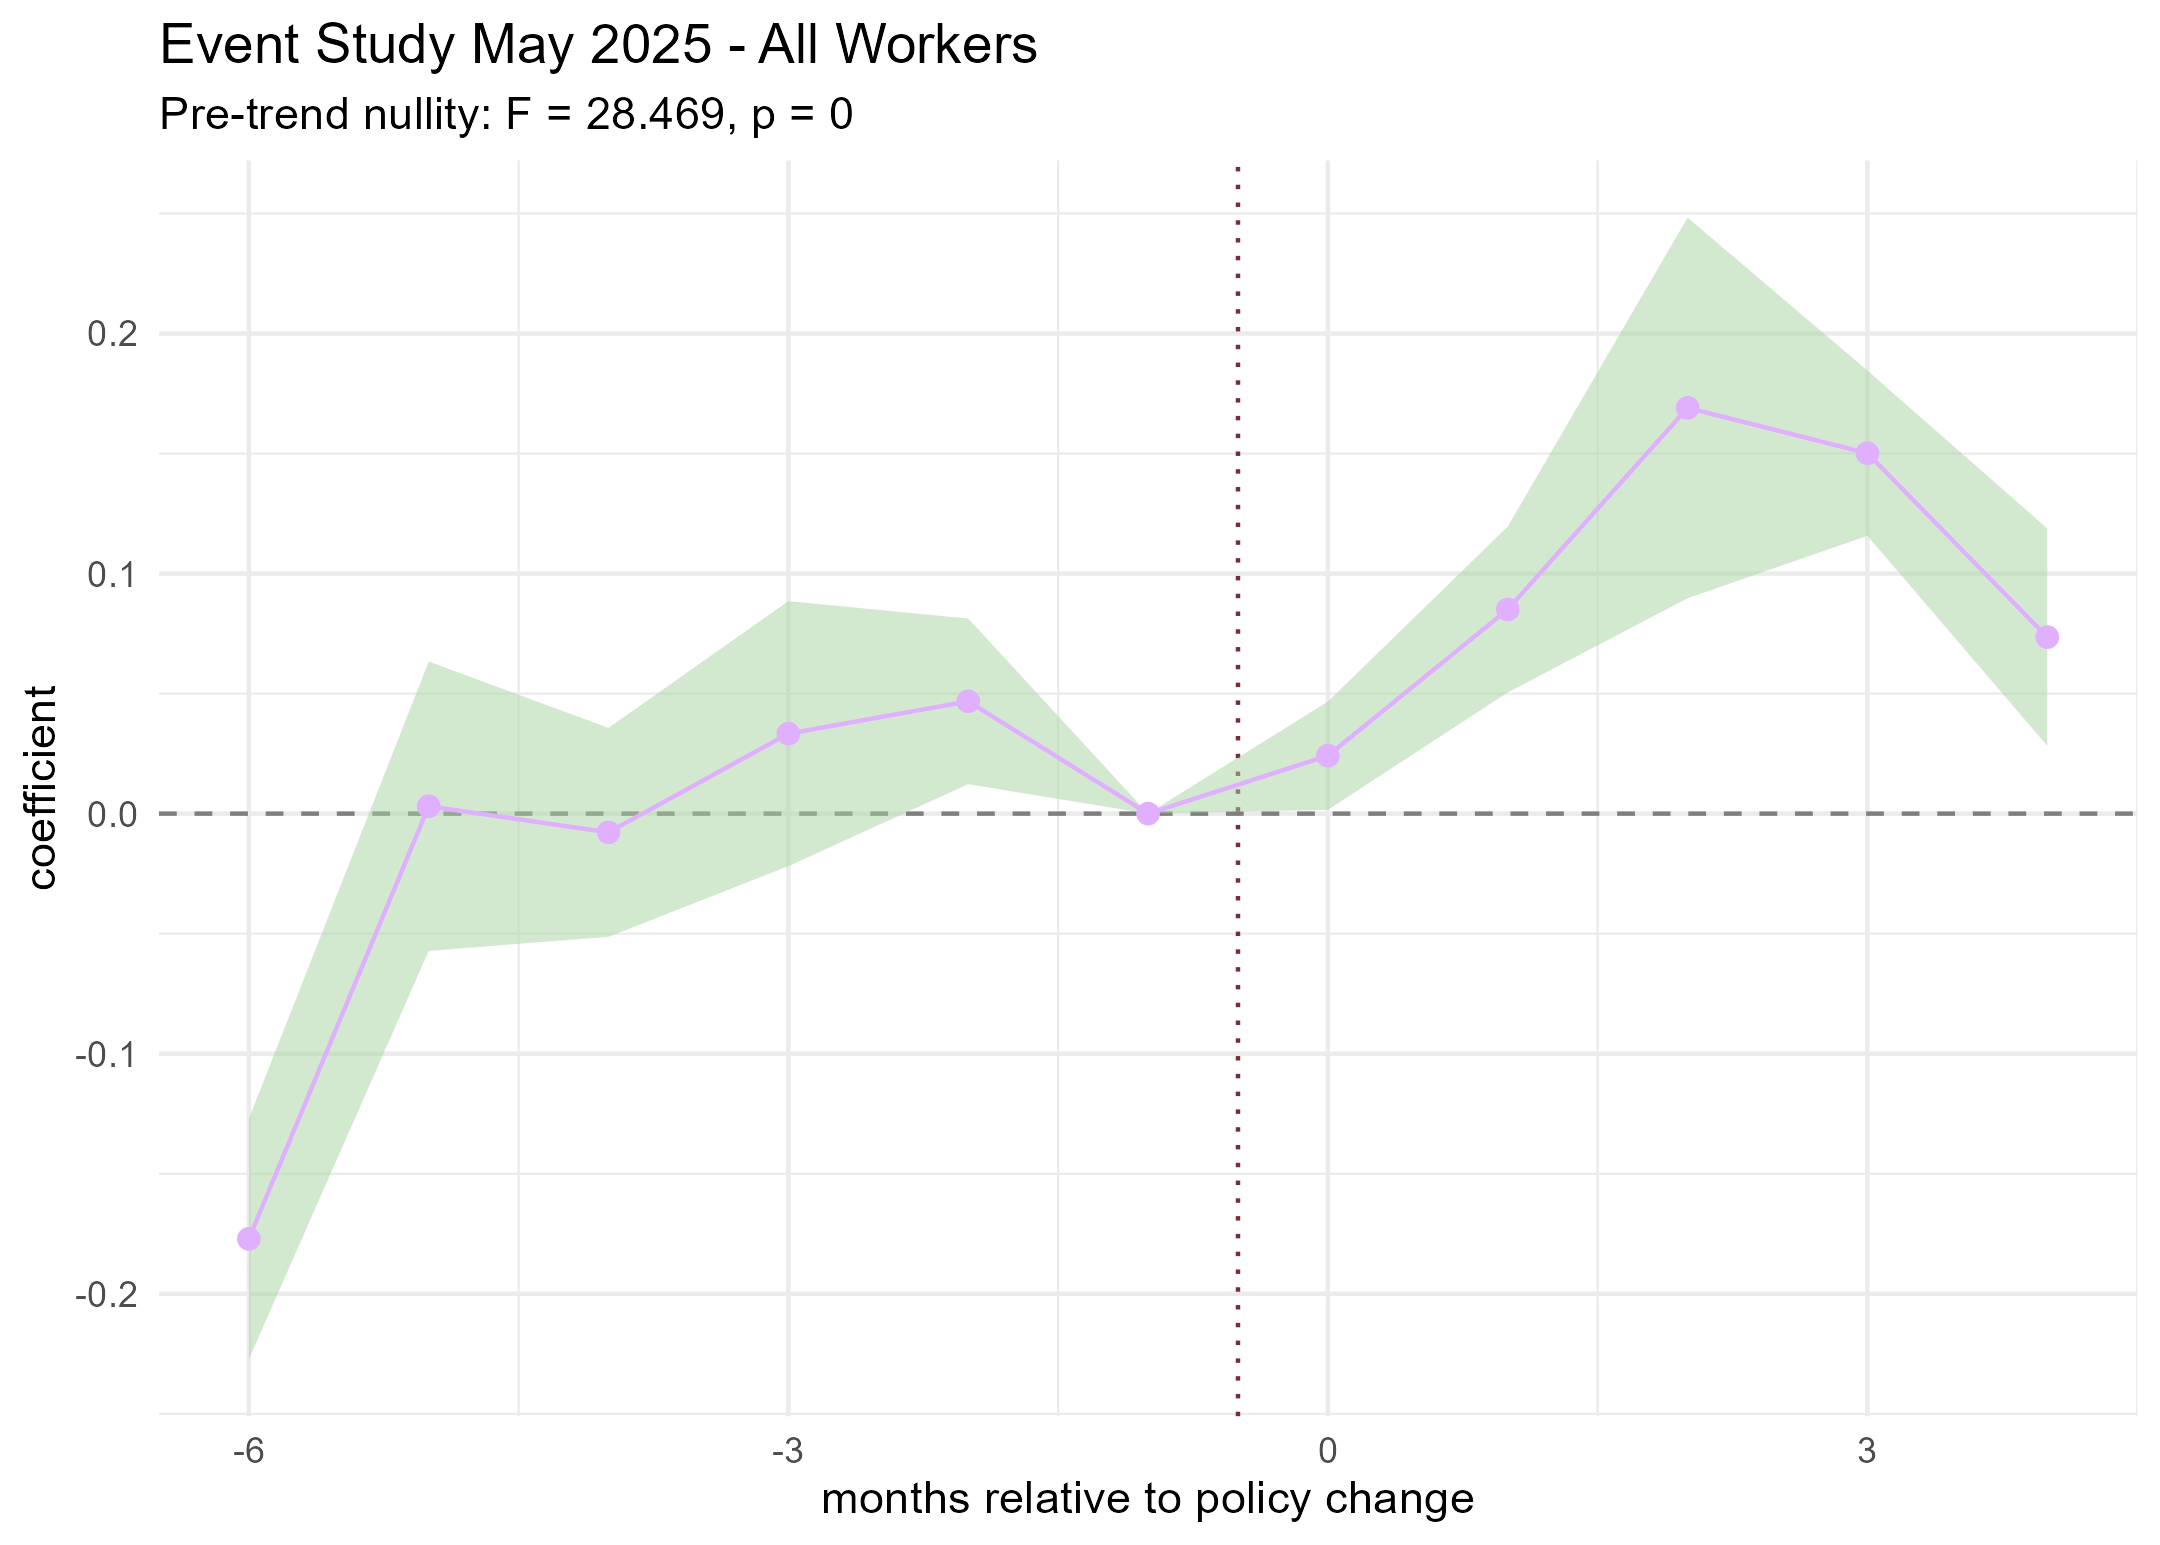
\includegraphics[width=\linewidth]{../../03 Output/DiD/event_study_2025.png}
\end{subfigure}\hfill
\begin{subfigure}{0.48\textwidth}
  \caption{French}
  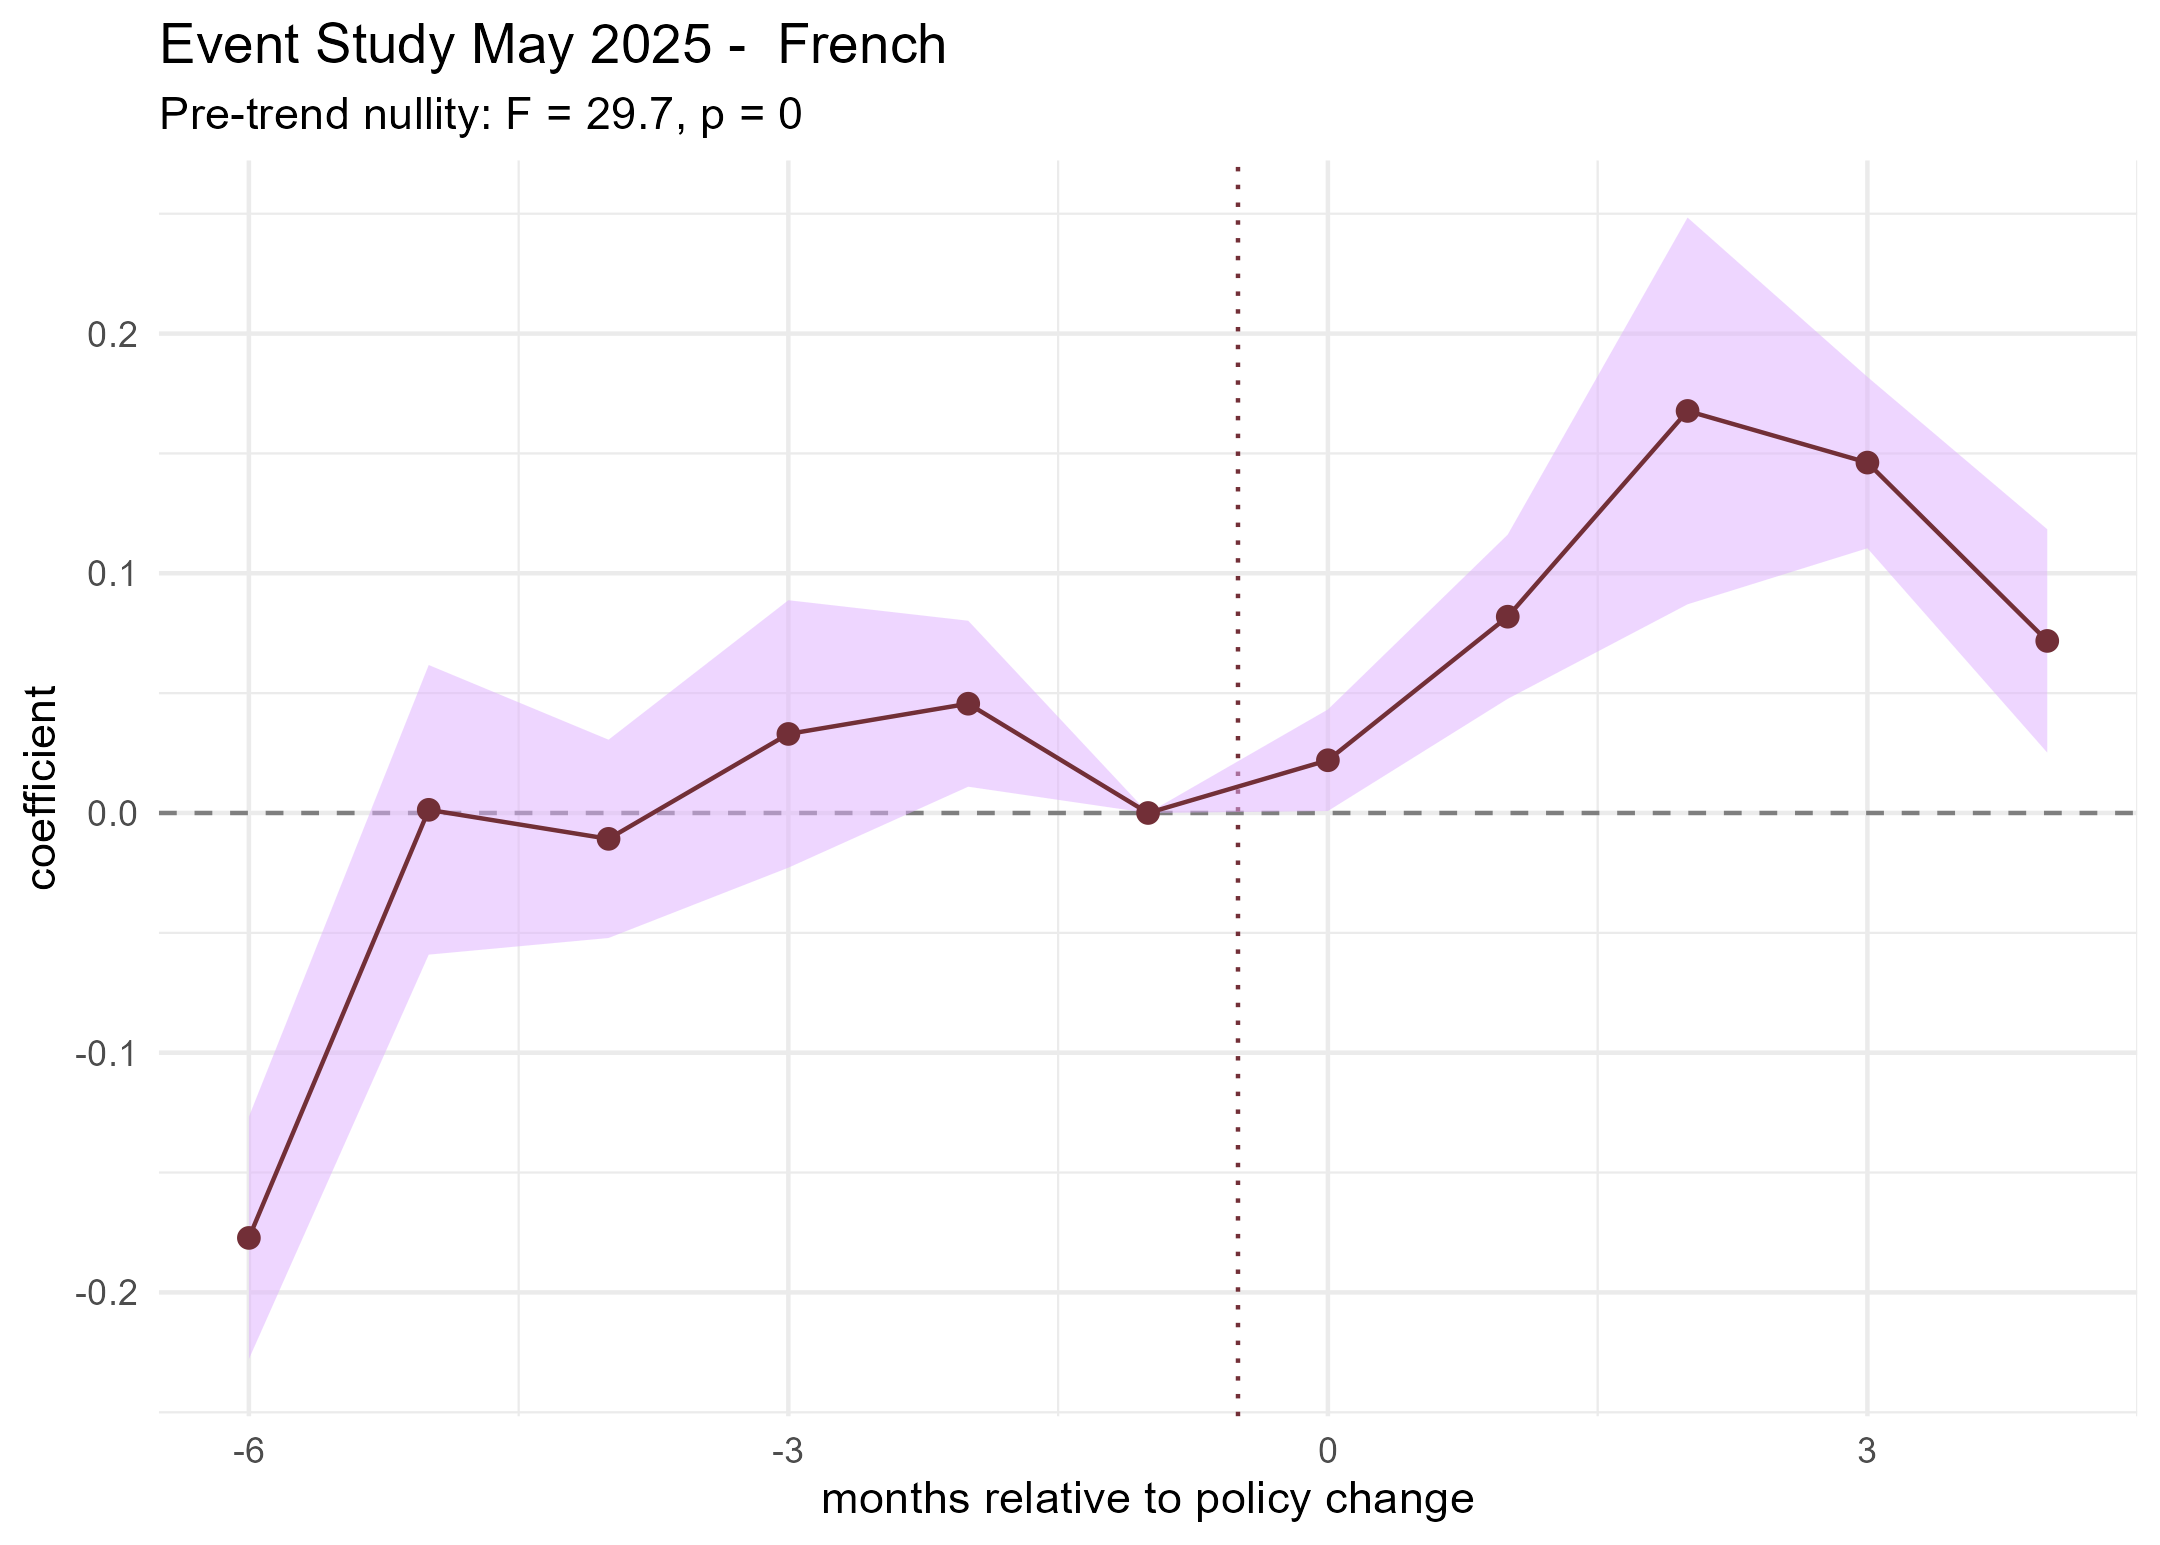
\includegraphics[width=\linewidth]{../../03 Output/DiD/event_study_french_2025.png}
\end{subfigure}
\par\medskip
\begin{subfigure}{0.48\textwidth}
  \caption{EEA}
  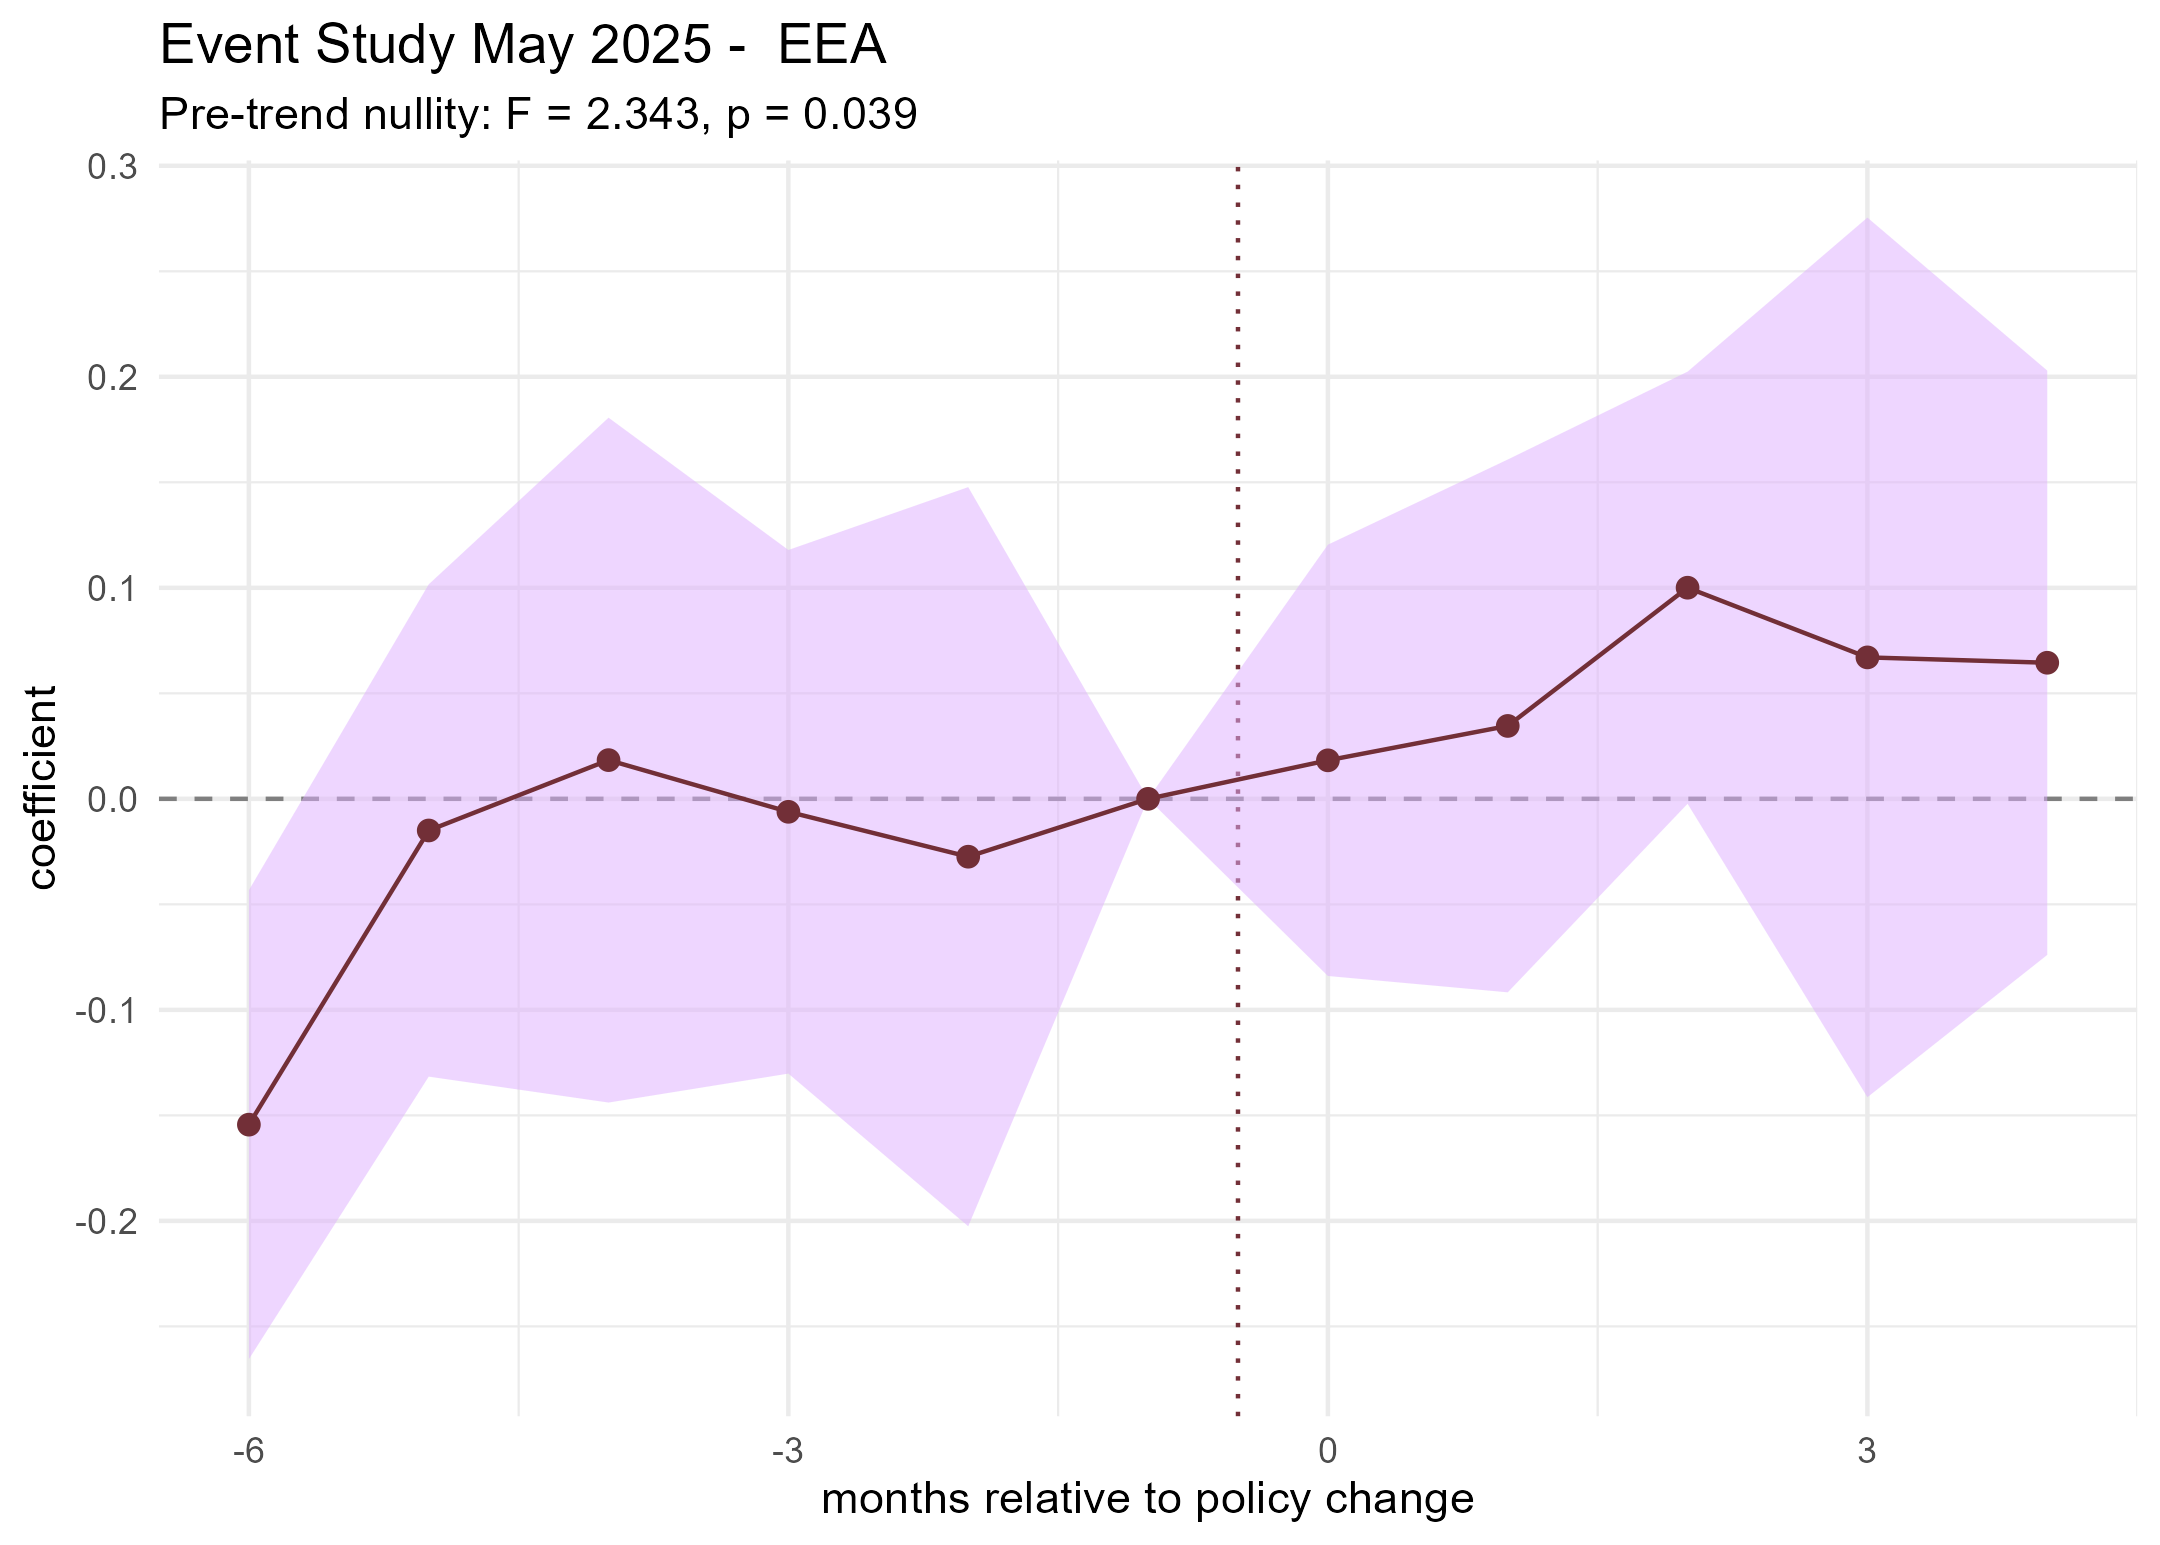
\includegraphics[width=\linewidth]{../../03 Output/DiD/event_study_eea_2025.png}
\end{subfigure}\hfill
\begin{subfigure}{0.48\textwidth}
  \caption{Non-EEA}
  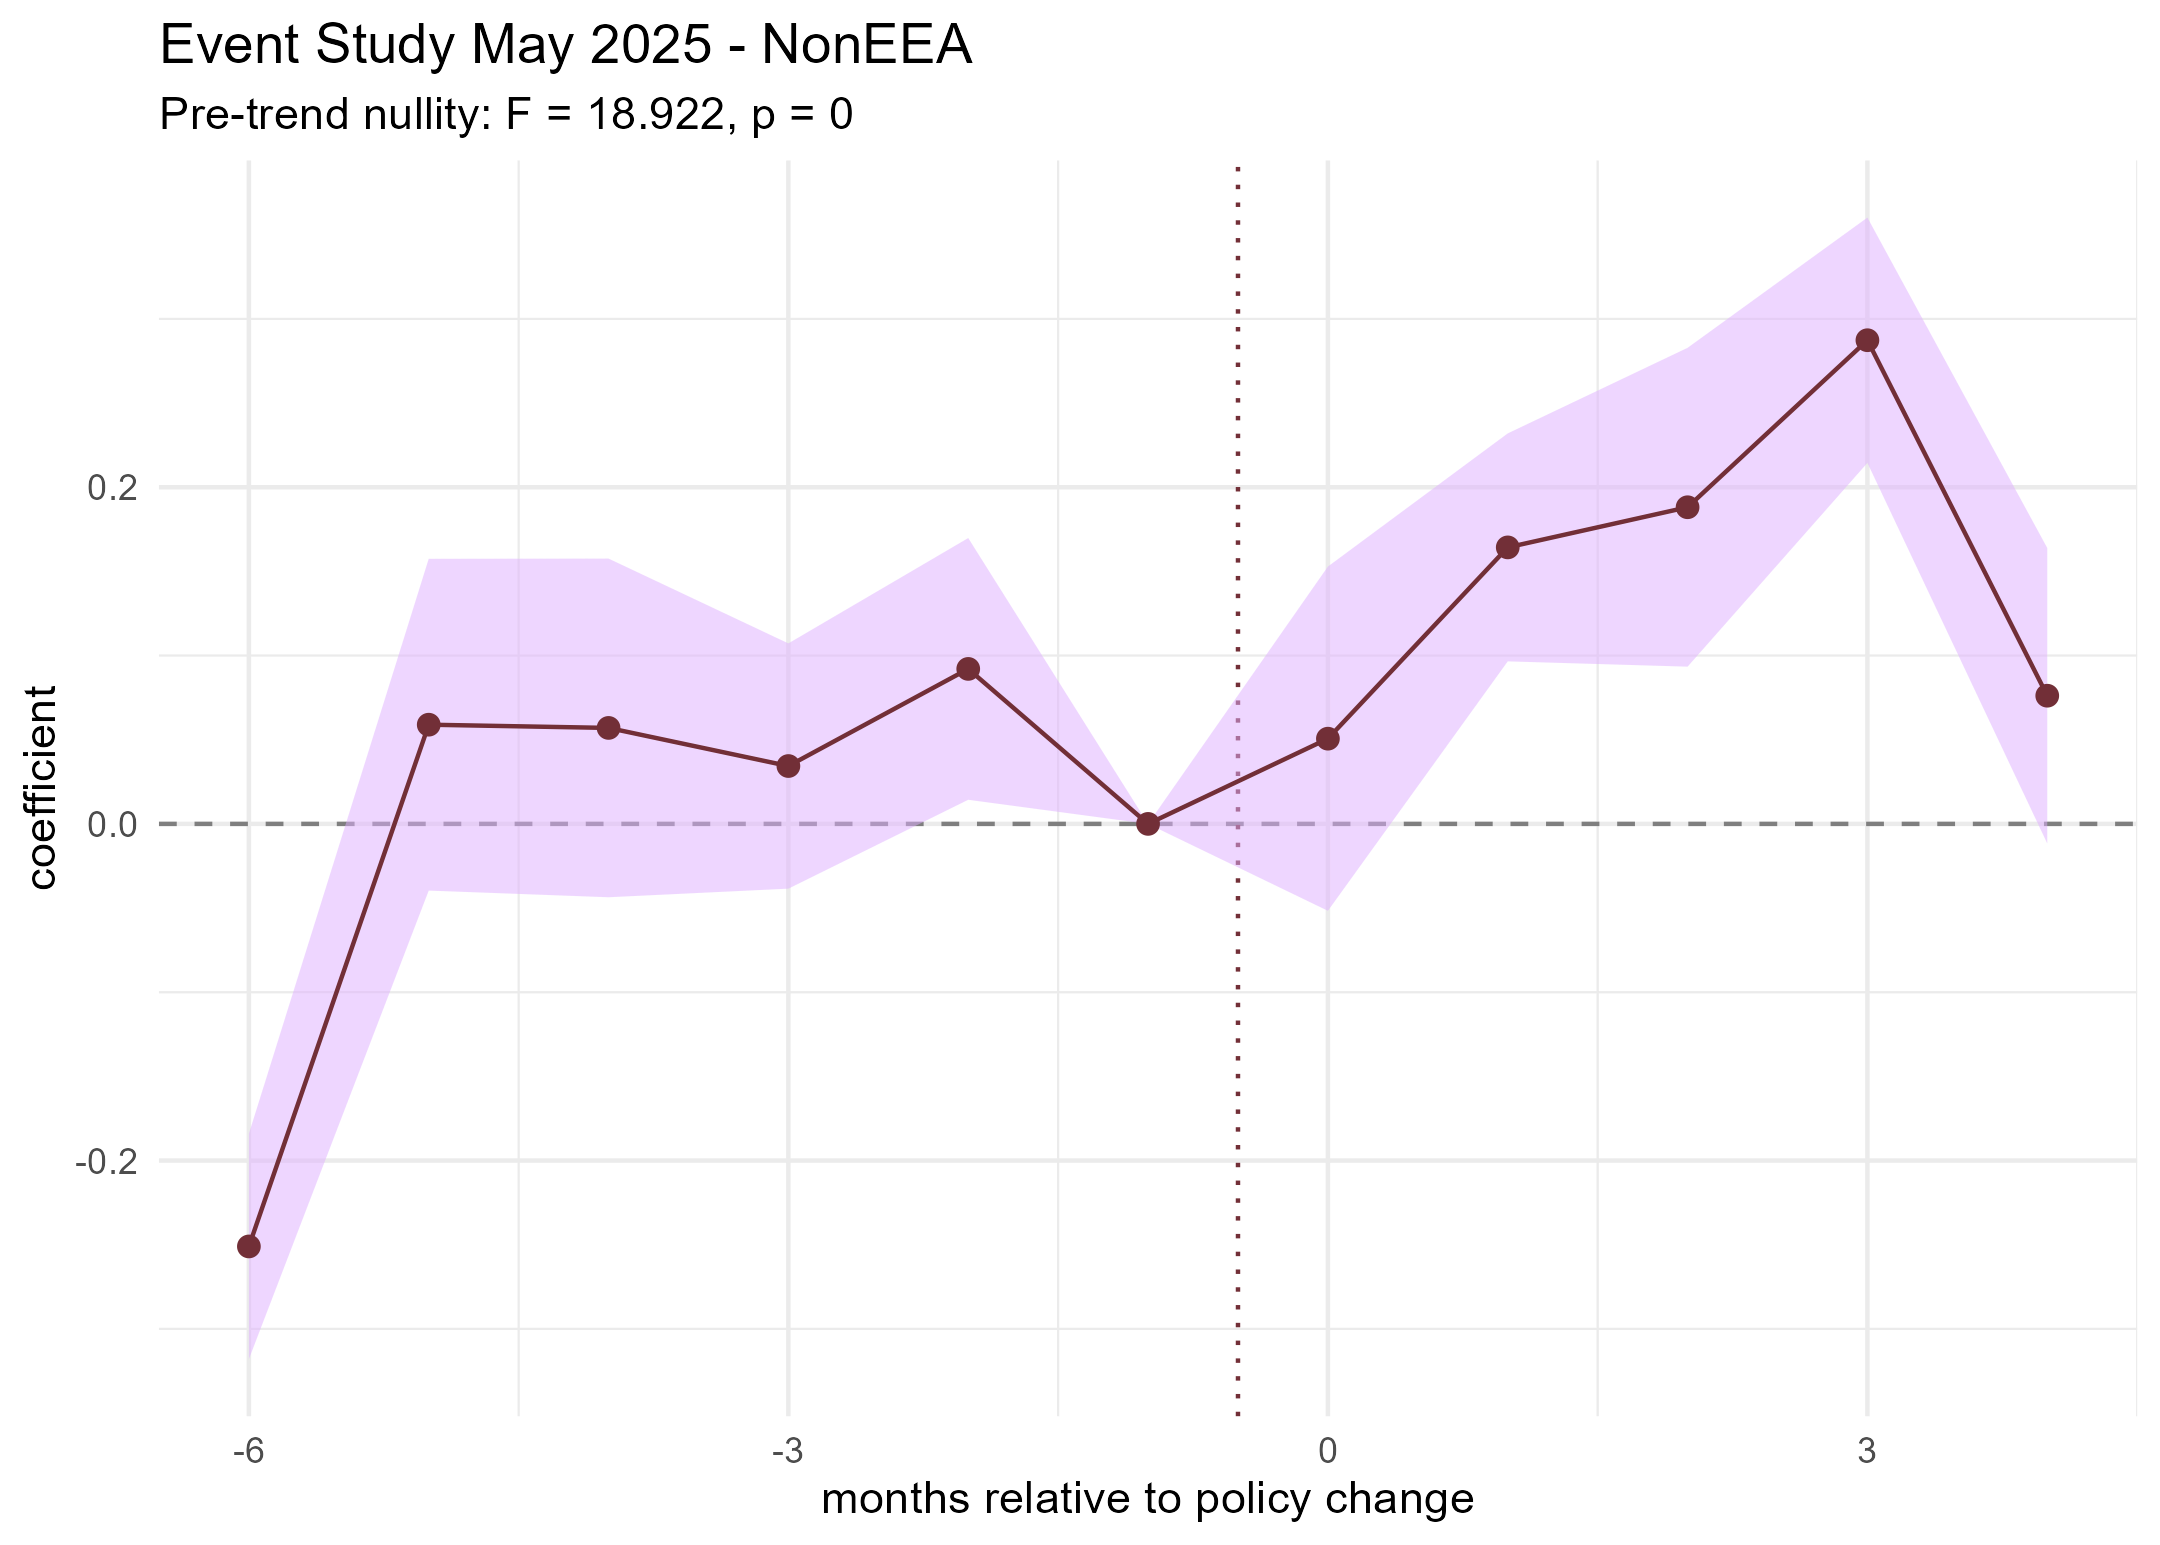
\includegraphics[width=\linewidth]{../../03 Output/DiD/event_study_non_eea_2025.png}
\end{subfigure}
\par\smallskip
{\footnotesize FE3 specification ($\mathtt{fap\_code \times year + region \times year}$), $\pm6$-month window. 95\% confidence intervals, SEs clustered at FAP level.}
\end{figure}

\begin{table}[h!]
\caption{2025 Reform (FE2)\label{tab:did2025_fe2}}
\centering
\setlength{\tabcolsep}{25pt}
\begin{tabular}{lrrrr}
 & \textit{all} & \textit{french} & \textit{EEA} & \textit{non-EEA} \\
\midrule
\midrule
Post & $0.006$ & $0.006$ & $-0.007$ & $0.031$ \\
 & (0.010) & (0.010) & (0.019) & (0.021) \\[2pt]
Treat$\,\times\,$Post & $-0.006$ & $-0.007$ & $0.022$ & $-0.001$ \\
 & (0.014) & (0.015) & (0.028) & (0.021) \\[2pt]
\midrule
Age & $-0.001$ & $-0.001$ & $-0.001$ & $-0.001$ \\
 & (0.000) & (0.000) & (0.001) & (0.001) \\[2pt]
Diploma & $0.004$ & $0.004$ & $-0.016$ & $0.018$ \\
 & (0.003) & (0.003) & (0.020) & (0.013) \\[2pt]
Part-time & $-0.802^{***}$ & $-0.802^{***}$ & $-0.687^{***}$ & $-0.904^{***}$ \\
 & (0.033) & (0.033) & (0.069) & (0.057) \\[2pt]
Education & $0.004$ & $0.004$ & $0.006$ & $0.002$ \\
 & (0.003) & (0.003) & (0.005) & (0.003) \\[2pt]
Male & $0.065^{**}$ & $0.065^{**}$ & $0.029$ & $0.079^{**}$ \\
 & (0.027) & (0.028) & (0.030) & (0.034) \\[2pt]
\midrule
Observations & 583{,}337 & 567{,}507 & 6{,}332 & 9{,}498 \\
\bottomrule
\multicolumn{5}{p{0.88\linewidth}}{\footnotesize Fixed effects: \texttt{fap\_code $\times$ region $\times$ year} (treatment level absorbed). SEs clustered at FAP level}\\
\end{tabular}
\end{table}

\clearpage
\section*{Appendix D - Cleaning Procedure}

\begin{center}
\small
\begin{tabular}{llll}
\textit{where}
 & \textit{script} & \textit{input} & \textit{output} \\
\midrule
CASD & \texttt{01 FH Cleaning.sas}             & FH raw           & \texttt{fh\_latest.csv}, \texttt{unique\_ids.csv} \\
CASD & \texttt{02 MMO Cleaning.sas}            & MMO raw          & \texttt{mmo\_latest.csv} \\
Outside & \texttt{01 build shortage list.R}       & PDF \textit{arrêtés}, DARES xls & \texttt{shortage\_list.csv} \\
CASD & \texttt{03 Shortage List + FAP PCS Match.R} & \texttt{shortage\_list.csv}, PCS-ESE ods & \texttt{fap\_to\_pcs.csv} \\
CASD & \texttt{04 Parquet + Final Cleaning.R}  & all CSVs         & \texttt{mmo\_latest\_wage.parquet} \\
CASD & \texttt{01 DiD.R}                       & all parquets     & analysis dataset \\
\bottomrule
\end{tabular}
\end{center}
\bigskip

\subsection*{Part 1: FH Cleaning \textnormal{\small(\texttt{01 FH Cleaning.sas})}}
\smallskip
\begin{itemize}
  \item \textit{Nationality restriction:} retain only spells where \texttt{NATION} corresponds to:
  \begin{center}
  \small
  \begin{tabular}{lll}
  \toprule
  Code & Country & Group \\
  \midrule
  01 & France & French (reference) \\
  24 & Serbia / Bosnia-Herz. & Non-EEA \\
  26 & Kosovo / Montenegro / N. Macedonia & Non-EEA \\
  29 & Turkey & Non-EEA \\
  27 & Croatia & EEA \\
  96 & Slovenia & EEA \\
  97 & Bulgaria & EEA \\
  98 & Romania & EEA \\
  19 & Greece & EEA \\
  02, 91--95 & Baltics, Hungary and Slavic Central Europe & EEA \\
  \bottomrule
  \end{tabular}
  \end{center}
  \smallskip

  \item \textit{Temporal restriction:} keep spells with \texttt{datins} $\geq$
  1 January 2019 to ensure at least two pre-treatment years before the April 2021 reform.   \smallskip

  \item \textit{Education:} \texttt{NIVFOR} alphanumeric codes
  (\texttt{AFS}, \texttt{CP4}, \ldots, \texttt{NV1}) are mapped to 0-9 scale (\texttt{formation}) for use as a continuous control.   \smallskip

  \item \textit{One row per worker:} FH records unemployment spells. Multiple
  rows may exist per \texttt{id\_force}. 
  \begin{itemize}
    \item Workers with a single spell: kept as-is.
    \item Workers with multiple spells: the row with the latest \texttt{datins}
    is retained for the sake of time. Matching each contract to the relevant characteristics would have taken too much time, and given that not many people were involved we decided to accept this error.
  \end{itemize}   \smallskip

  \item \textit{ID export:} distinct \texttt{id\_force} values are exported to
  \texttt{unique\_ids.csv} and used as a hash reference.
\end{itemize}
\bigskip

\subsection*{Part 2: MMO Cleaning \textnormal{\small(\texttt{02 MMO Cleaning.sas})}}
\smallskip
\begin{itemize}
  \item \textit{ID filter:} hash join on \texttt{unique\_ids} restricts MMO
  to workers present in FH. This is necessary to attach nationality and
  controls from FH.
  \smallskip
  \item \textit{Contract filters:} applied to each annual file 2019-2025:
  \begin{itemize}
    \item drop rows with missing \texttt{L\_Contrat\_SQN}, as these contracts have ended and are recorded in other vintages.
    \item Drop contracts starting before 2019.
    \item Drop contracts shorter than 31 days. Very short spells are either \textit{période d'essai} or do not reflect stable employment.
  \end{itemize}
  \smallskip
  \item \textit{Deduplication across annual files:} the same contract can
  appear in multiple annual MMO files (once per year until its end date),
  with later files potentially containing corrections. A contract-level
  index is built across all years. For each \texttt{L\_Contrat\_SQN},
  only the most recent vintage is kept.
  \smallskip
  \item \textit{Policy timing dummies:} binary indicators are created for
  contract start after each reform date: \texttt{post\_apr2021} (1 Apr 2021),
  \texttt{post\_jan2024} (29 Jan 2024), \texttt{post\_mar2024} (1 Mar 2024),
  \texttt{post\_apr2025} (1 Apr 2025), \texttt{post\_may2025} (21 May 2025).
  Symmetric two-year DSN recency windows were also created for robustness checks, but we did not use them. 
\end{itemize}
\bigskip

\subsection*{Part 3. Shortage List Construction and FAP-PCS Matching
\textnormal{\small(\texttt{01 build shortage list.R},
\texttt{03 Shortage List + FAP PCS Match.R})}}
\smallskip
\begin{itemize}
  \item The four \textit{arrêtés} (2008, 2021, 2024, 2025) are parsed from
  PDF. Each FAP code is mapped to PCS-2003 codes via a DARES
  correspondence table. Note that this matching relates only to treated occupations.
  \smallskip
  \item The 2024 amendment is applied as a set of targeted removals and
  additions to the 2021 list. Delisting and relisting flags are constructed.
 \smallskip
  \item On the CASD, we verify that the PCS codes in
  \texttt{shortage\_list.csv} align with the PCS-ESE codes recorded in  (\texttt{Table\_passage\_FAP\_PCS-ESE.ods}), which is a table we found in the CASD, and in MMO. A mistake occurred here: we did not detect that the .ODS table present on the CASD did not fully align with the MMO. 
  \smallskip
  \item The FAP-PCS crosswalk and the treatment status assignment are not merged at this stage.
\end{itemize}
\bigskip

\subsection*{Part 4. Wage Harmonisation and Geographic Scope
\textnormal{\small(\texttt{04 Parquet + Final Cleaning.R})}}
\smallskip
\begin{itemize}
  \item \textit{format conversion:} all CSVs are converted to Parquet.
  Subsequent operations run via DuckDB without loading files into memory.
  \smallskip
  \item \textit{wage harmonisation.} a standardised \texttt{monthly\_wage}
  is constructed from \texttt{salaire\_base}, \texttt{ModeExercice}, and
  \texttt{salaire\_base\_mois\_complet}:
  \begin{itemize}
    \item \textit{part-time}: \texttt{ModeExercice} $\in \{20,30,40,41,42\}$,
    or \texttt{ModeExercice = 99} with \texttt{salaire\_base} $< 1{,}498$
    (2019 SMIC monthly gross).
    \item If part-time and \texttt{salaire\_base\_mois\_complet = 1}:
    \texttt{monthly\_wage = salaire\_base} (already full-month equivalent).
    \item If full-time and \texttt{salaire\_base\_mois\_complet = 0}:
    \texttt{monthly\_wage = salaire\_base} $\times 30.4375\,/\,\text{contract days}$.
    \item All other combinations are set to missing and excluded from regressions.
  \end{itemize}
  \smallskip
  \item \textit{Geographic restriction:} contracts are assigned to the
  13 metropolitan regions via a postal-code prefix crosswalk. Contracts
  with \texttt{CP} mapping to \textit{Outre-Mer} (prefixes 97-98) or
  abroad are dropped, as the shortage lists apply only to metropolitan France.
\end{itemize}
\bigskip

\subsection*{Part 5. Final Merge and Treatment Assignment
\textnormal{\small(\texttt{01 DiD.R})}}
\smallskip
\begin{itemize}
  \item MMO and FH are joined on \texttt{id\_force}. 
\smallskip
  \item The shortage list is joined on \texttt{pcs\_code} and
  \texttt{region\_contract = region}. Treatment indicators
  are \texttt{COALESCE}d to 0 for unmatched contracts, which form
  the control group.
  \item Age (\texttt{contract\_year} $-$ birth year), a male dummy,
  a diploma dummy, and experience in months are derived at this stage.
\end{itemize}

\end{document}



